\documentclass[english, bachelorthesis]{mmt}

\usepackage[all]{nowidow}
\usepackage{mathptmx}
\usepackage{graphicx}
\usepackage{times}
\usepackage{subfig}
\usepackage{float}
\usepackage[utf8]{inputenc}
\usepackage{listings}
\usepackage{makecell}
\usepackage[toc,page]{appendix}
\usepackage{hyperref}
\hypersetup{
    colorlinks,
    citecolor=black,
    filecolor=black,
    linkcolor=black,
    urlcolor=black
}
\usepackage{breakurl}

\usepackage{amsmath}
\usepackage[autostyle,german=guillemets]{csquotes}
\usepackage[useregional]{datetime2}

\usepackage{verbatim}

\newcommand{\detailtexcount}[1]{%
  \immediate\write18{texcount -merge -sum #1.tex > #1.wcdetail}%
  \verbatiminput{#1.wcdetail}%
}

\newcommand*{\enq}{\enqoute}

% moved to cls file. use \selectthesislanguage to switch to default language
%\usepackage[english,ngerman]{babel}

\usepackage{acronym}
\usepackage{abbrevs}
%% the following solves a bug in the abbrevs package, that adds an empty
%% space after the abbrev
\makeatletter
\renewcommand\maybe@space@{%
  % \@tempswatrue % <= this is in the original
  \maybe@ictrue % <= this is new
  \expandafter   \@tfor
    \expandafter \reserved@a
    \expandafter :%
    \expandafter =%
                 \nospacelist
                 \do \t@st@ic
  % \if@tempswa % <= this is in the original
  \ifmaybe@ic % <= this is new
    \space
  \fi
}
\makeatother
%%

\usepackage{color}
\definecolor{lightgray}{rgb}{.9,.9,.9}
\definecolor{darkgray}{rgb}{.4,.4,.4}
\definecolor{purple}{rgb}{0.65, 0.12, 0.82}
\lstdefinelanguage{JavaScript}{
  keywords={await, break, case, catch, continue, debugger, default, delete, do, else, false, finally, for, function, if, in, instanceof, new, null, return, switch, this, throw, true, try, typeof, var, let, const, void, while, with},
  morecomment=[l]{//},
  morecomment=[s]{/*}{*/},
  morestring=[b]',
  morestring=[b]",
  ndkeywords={class, export, boolean, throw, implements, import, this},
  keywordstyle=\color{blue}\bfseries,
  ndkeywordstyle=\color{darkgray}\bfseries,
  identifierstyle=\color{black},
  commentstyle=\color{purple}\ttfamily,
  stringstyle=\color{red}\ttfamily,
  sensitive=true
}

\lstset{
   language=JavaScript,
   backgroundcolor=\color{lightgray},
   extendedchars=true,
   basicstyle=\footnotesize\ttfamily,
   showstringspaces=false,
   showspaces=false,
   numbers=left,
   numberstyle=\footnotesize,
   numbersep=9pt,
   tabsize=2,
   breaklines=true,
   showtabs=false,
   captionpos=b
}

\usepackage[authordate,bibencoding=auto,strict,noibid,backend=bibtex]{biblatex-chicago}
\bibliography{bibliography}

%% Add configuration options
\newabbrev{\authorname}{Martin Sonnberger}
\newabbrev{\authormail}{msonnberger.mmt-b2020@fh-salzburg.ac.at}
\newabbrev{\titlename}{Detecting and Visualizing Delay Hotspots in Vienna's Public Transport Network}
\newabbrev{\advisor}{Andreas Bilke, MSc}
%\newabbrev{\secondadvisor}{Titel Vorname Nachname}
\newabbrev{\thesisdate}{\DTMdisplaydate{2023}{5}{2}}
\newabbrev{\thesisrepo}{https://gitlab.mediacube.at/fhs45907/bachelor-thesis}
\newabbrev{\keywordsenglish}{word1, word2, word3}
\newabbrev{\keywordsgerman}{wort1, wort2, wort3}


%% Paper title.

\title{\titlename}

%% This is how authors are specified in the conference style

%% Author 
\author{ \authorname\\ \scriptsize \authormail \\ \scriptsize 
\ifmmtlanguagegerman FH Salzburg \else Salzburg University of Applied Sciences \fi
}

%% A teaser figure can be included as follows, but is not recommended since
%% the space is now taken up by a full width abstract.
%\teaser{
%  \includegraphics[width=1.5in]{sample.eps}
%  \caption{This can be a teaser image of the thesis.}
%}

%% Abstract section for paper format.
\abstract{
    \ifmmtlanguagegerman 
        \selectlanguage{ngerman}
        Um die Fahrgastzahlen und die Kundenzufriedenheit in öffentlichen Verkehrsnetzen zu erhöhen, müssen Verkehrsbetriebe verschiedene Maßnahmen ergreifen, um eine attraktive Alternative zu anderen Verkehrsmitteln zu bieten. Neben dem Angebot eines umfangreichen Netzes und der Verbesserung der Infrastruktur ist eine dieser Maßnahmen die Verringerung von Verspätungen und die Bereitstellung zuverlässiger Verbindungen. Um Verspätungen effizient zu reduzieren, ist es wünschenswert, Hotspots im Netz zu erkennen, an denen die meisten Verspätungen auftreten. Ziel dieser Arbeit ist es, Abfahrtsdaten zu analysieren, um potenzielle Hotspots zu finden und zu untersuchen, ob sich diese Hotspots an Umsteigeknoten und Endstationen befinden. Zu diesem Zweck wurden über einen Zeitraum von 30 Tagen Abfahrtsdaten im Wiener Nahverkehrsnetz erhoben. Nach einem Überblick über frühere Untersuchungen in anderen Städten werden die Ergebnisse der Analyse und mögliche Gründe für die Ergebnisse in dieser Arbeit diskutiert. Zusätzlich werden dem Leser Visualisierungen der gesammelten Verspätungsdaten präsentiert, um die Ergebnisse in einer leicht verständlichen Form darzustellen.
    \else 
        \selectlanguage{english}
        In order to increase passenger numbers and customer satisfaction in public transport networks, transit authorities have to take various measures to provide an attractive alternative to other forms of transport. Besides offering an extensive network and improving infrastructure, one of those measures is reducing delays and providing reliable services. To efficiently reduce delays, it is desirable to detect hotspots in the network where delays occur the most. This thesis aims to analyze departure data to find potential hotspots and answer whether those hotspots are at transfer hubs and terminal stations. To do so, departure data in Vienna's public transport network was collected over 30 days. After reviewing previous research conducted in other cities, the results of the analysis and possible reasons for the results will be discussed in this thesis. Additionally, visualizations of the collected delay data will be presented to the reader in order to show the results in a more easy-to-understand way.
    \fi
}

\usepackage[super]{nth}
\usepackage{booktabs}
\usepackage{cleveref}

%%%%%%%%%%%%%%%%%%%%%%%%%%%%%%%%%%%%%%%%%%%%%%%%%%%%%%%%%%%%%%%%
%%%%%%%%%%%%%%%%%%%%%% START OF THE PAPER %%%%%%%%%%%%%%%%%%%%%%
%%%%%%%%%%%%%%%%%%%%%%%%%%%%%%%%%%%%%%%%%%%%%%%%%%%%%%%%%%%%%%%%%

\begin{document}
% TODO switch for english, german
\selectthesislanguage

\pagenumbering{gobble}

 % group open
\ifmmtpaper
    \begingroup 
    % is required because paper template messes with sizes
    \fontsize{12}{18}\selectfont        
    \setlength{\parindent}{0pt}
    \setlength{\parskip}{5pt plus 2pt minus 1pt}
    \sectionfont{\fontsize{14}{15}\selectfont}
\fi

\ifmmtreviewversion
    \titlename
\else
    \begin{titlepage}

% check if second advisor exists
\newcommand{\printsecondadvisor}[1]{%
  \ifcsname#1\endcsname%
  \ifmmtlanguagegerman Zweitbetreuer*in: \else Second Advisor: \fi \secondadvisor 
  \else%
    
  \fi%
}

\ifmmtmasterthesis

    
    % \begin{center}
    %     \Huge{ 
    %     	\textbf{\ifmmtlanguagegerman Masterarbeit \else Master Thesis \fi}
    %     }
    % \end{center}
    
    \newpage
    
    \thispagestyle{empty}
    
    \hfill 
\includegraphics[height=1.5cm]{images/FHSLogo.jpg}
    
    \vspace*{2cm}
    
    \Large{
    \titlename
    
    \vspace*{1cm}
    
    \ifmmtlanguagegerman
    Masterarbeit zur Erlangung des akademischen Grades
    \else
    Master thesis in partial fulfilment of the requirements for\\ the degree of 
    \fi
    
    \vspace*{0.5cm}
    
    \textit{Master of Science}
    }
    
    
    \vspace*{1.5cm}
    {\large
    \ifmmtlanguagegerman Autor*in: \else Author: \fi \authorname
    }
    \vfill
    
    {\normalsize
    \ifmmtlanguagegerman
    Vorgelegt am FH-Masterstudiengang MultiMediaTechnology, Fachhochschule Salzburg
    \else
    Submitted to the Master degree program MultiMediaTechnology, Salzburg University of Applied Sciences
    \fi
    
    
    \vspace*{1cm}
    
    \ifmmtlanguagegerman Betreuer*in: \else Advisor: \fi
    \advisor
    \\    
    \printsecondadvisor{secondadvisor}
    
    \vfill
    
    Salzburg, \ifmmtlanguagegerman Österreich, \else Austria, \fi  \thesisdate
    }

\else % Bachelor thesis title page

    \begin{center}
    
    
\includegraphics[width=5cm]{images/FHSLogo.jpg}


    \vspace*{4cm}
    
    \fontsize{20.79}{18pt}{\selectfont        
    %\Large{
    	\textit{\textbf{\titlename}}
    %}
    }
    
    \vspace*{4cm}
    
    \fontsize{20.79}{18pt}{%\large{
    \ifmmtlanguagegerman
      \textbf{ \ifmmtpaper Seminararbeit \else Bachelorarbeit \fi }
    \else
        \textbf{ \ifmmtpaper Seminararbeit \else Bachelor Thesis \fi }
    \fi
    }
    
    
    \end{center}
    
    \vfill
    
    %\begin{tabular}{ll}
    \ifmmtlanguagegerman Autor*in: \else Author: \fi  \authorname  \\
    \ifmmtlanguagegerman Betreuer*in: \else Advisor: \fi \advisor \\
    Repository: \thesisrepo \\
    \printsecondadvisor{secondadvisor}
    
    Salzburg, \ifmmtlanguagegerman Österreich, \else Austria, \fi \thesisdate
    
    
    
    % uncomment the following 3 lines for an optional lock flag, max. 2 years!
    %\hfill
    %\color{red}
    %\framebox{Sperrvermerk bis 20/01/2012}

\fi

\end{titlepage}
       
\fi

    \onecolumn           
    
    \pagenumbering{roman}
    
\ifmmtpaper % does not need affidavit
\else \ifmmtreviewversion
      \else
        \newpage
        
\ifmmtlanguagegerman
\subsection*{Eidesstattliche Erklärung}


Ich erkläre hiermit eidesstattlich, dass ich die vorliegende Arbeit selbstständig und ohne fremde Hilfe verfasst, und keine anderen als die angegebenen Quellen und Hilfsmittel benutzt habe. Weiter versichere ich hiermit, dass ich die den benutzten Quellen wörtlich oder inhaltlich entnommenen Stellen als solche kenntlich gemacht habe.

Die Arbeit wurde bisher in gleicher oder ähnlicher Form keiner anderen Prüfungskommission weder im In- noch im Ausland vorgelegt und auch nicht veröffentlicht.

\else

\subsection*{Affidavit}

I herewith declare on oath that I wrote the present thesis without the help of third persons and without using any other sources and means listed herein; I further declare that I observed the guidelines for scientific work in the quotation of all unprinted sources, printed literature and phrases and concepts taken either word for word or according to meaning from the Internet and that I referenced all sources accordingly.

This thesis has not been submitted as an exam paper of identical or similar form, either in Austria or abroad and corresponds to the paper graded by the assessors.

\fi

\vspace*{3cm}

%{\bf \thesisdate{}}


\hfill

\ifmmtlanguagegerman
$\overline{Datum \hspace{2cm}}$ \hfill $\overline{{Unterschrift}\hspace{3cm}}$

\vspace*{1cm}

\hfill $\overline{{Vorname\hspace{2cm}Nachname}}$
 
 \else

 $\overline{Date \hspace{2cm}}$ \hfill $\overline{{Signature}\hspace{4cm}}$

\vspace*{1cm}

 \hfill $\overline{{First~Name\hspace{2cm}Last~Name}}$
 \fi

  % comment out for expose
      \fi
\fi
% group closing
\ifmmtpaper
\endgroup
\fi


\ifmmtpaper \else  % paper does not need this stuff
    
    \newpage
    \selectlanguage{ngerman}
    \section*{Kurzfassung}
    Um die Fahrgastzahlen und die Kundenzufriedenheit in öffentlichen Verkehrsnetzen zu erhöhen, müssen Verkehrsbetriebe verschiedene Maßnahmen ergreifen, um eine attraktive Alternative zu anderen Verkehrsmitteln zu bieten. Neben dem Angebot eines umfangreichen Netzes und der Verbesserung der Infrastruktur ist eine dieser Maßnahmen die Verringerung von Verspätungen und die Bereitstellung zuverlässiger Verbindungen. Um Verspätungen effizient zu reduzieren, ist es wünschenswert, Hotspots im Netz zu erkennen, an denen die meisten Verspätungen auftreten. Ziel dieser Arbeit ist es, Abfahrtsdaten zu analysieren, um potenzielle Hotspots zu finden und zu untersuchen, ob sich diese Hotspots an Umsteigeknoten und Endstationen befinden. Zu diesem Zweck wurden über einen Zeitraum von 30 Tagen Abfahrtsdaten im Wiener Nahverkehrsnetz erhoben. Nach einem Überblick über frühere Untersuchungen in anderen Städten werden die Ergebnisse der Analyse und mögliche Gründe für die Ergebnisse in dieser Arbeit diskutiert. Zusätzlich werden dem Leser Visualisierungen der gesammelten Verspätungsdaten präsentiert, um die Ergebnisse in einer leicht verständlichen Form darzustellen.
    \ifmmtmasterthesis
    
    \vspace*{0.5cm} 
    \textbf{Schlüsselwörter:~} \keywordsgerman
    \fi
    \newpage
    \selectlanguage{english}
    \section*{Abstract}
    In order to increase passenger numbers and customer satisfaction in public transport networks, transit authorities have to take various measures to provide an attractive alternative to other forms of transport. Besides offering an extensive network and improving infrastructure, one of those measures is reducing delays and providing reliable services. To efficiently reduce delays, it is desirable to detect hotspots in the network where delays occur the most. This thesis aims to analyze departure data to find potential hotspots and answer whether those hotspots are at transfer hubs and terminal stations. To do so, departure data in Vienna's public transport network was collected over 30 days. After reviewing previous research conducted in other cities, the results of the analysis and possible reasons for the results will be discussed in this thesis. Additionally, visualizations of the collected delay data will be presented to the reader in order to show the results in a more easy-to-understand way.
    \ifmmtmasterthesis
        
    \vspace*{0.5cm} 
    \textbf{Keywords:~} \keywordsenglish
    \fi
    \selectthesislanguage
    
    \newpage
    \tableofcontents
    
    \newpage
    \listoffigures
    \lstlistoflistings
    \listoftables
    \ifmmtlanguagegerman
\section*{Abkürzungsverzeichnis}
\else
\section*{Abbreviations and Acronyms}
\fi

% use as \ac{AR} in the text in body.tex and you don't have to think about
% introducing acronyms anymore correctly at the first mention in the text.
% do not use \ac in the Abstract/Kurzfassung. Otherwise, acronyms must be
% reintroduced in the main text
%
% if you want to use the acronym package for the paper template
% define the acronyms using acrodef and without the acronym environment
% \acrodef{AR}{Augmented Reality} somewhere in body.tex. this file
% will not be included when using the paper template.
\begin{acronym}
	\acro{API}{Application Programming Interface}
	\acro{CSV}{comma-separated values}
	\acro{FPTF}{Friendly Public Transport Format}
	\acro{GTFS}{General Transit Feed Specification}
	\acro{HAFAS}{HaCon-Fahrplan-Auskunfts-System}
	\acro{JSON}{JavaScript Object Notation}
	\acro{RDBMS}{relational database management system}
	\acro{SQL}{Structured Query Language}
	\acro{VOR}{Verkehrsverbund Ost-Region}
\end{acronym}

    
\fi


\mmtcolumnmode % switch back to column formatting of stylesheet

\maketitle % used for paper formatting

\ifmmtpaper\else
\pagestyle{headings}
\fi
\pagenumbering{arabic}


% put environments that should be ignored by texcount here, e.g., here lstlisting for code

%TC:envir lstlisting [] ignore
\graphicspath{ {./images/} }

\section{Introduction}

Good public transportation is one of the most important factors for quality of life in any big city. A study by the European Union found that after frequency, reliability is the second biggest contributing factor to passenger satisfaction with public transport \autocite[66]{eu-2020}. With the European Union's commitment to achieving 55\% less greenhouse gas emission in comparison to 1990, it is of high importance to increase both usage of and satisfaction with public transport. In Vienna, Austria both of these numbers are already at very high levels with 55\% of people using the public transport network on a typical day and 95\% average passenger satisfaction, the best value among capital cities in the EU \autocite[61]{eu-2020}. To be able to reduce delays and thus increase reliability, one has to first identify areas where delays occur most often and to the largest extent. After identifying these areas, possible reasons for occurring delays have to be explored, considering both internal and external reasons \autocite[372]{van-oort-2015}. Only after both of these steps have been completed, effective measures can be researched and implemented.

The aim of this thesis is to identify said problem areas by collecting and analyzing departure data from the transport agency that operates metros, trams and buses in Vienna. Since raw numbers alone often do not provide an intuitive understanding of large data sets, different visualizations will be presented that aim to give the reader an easy-to-understand overview of potential delay hotspots. In particular, the hypothesis that delays occur more often at transfer hubs and terminal stations will be investigated. At transfer hubs, passenger volume is the highest which can lead to increased dwell times and thus delays. At terminal stations on the other hand, delays that occurred at the beginning of a trip can accumulate and therefore form delay hotspots.

The thesis is structured as follows. \Cref{section:related-work} presents previous research and different formats of public transport data that are available in Vienna. \Cref{sec:implementation} first explains some relevant information about the network itself and continues to describe the data collection process in detail. For this process, a custom script was written that persisted the necessary data over a duration of 30 days. Next, the results of the conducted data analysis are presented, highlighting different aspects in varying levels of detail, starting with network-wide analysis and continuing with a closer look at single lines and stations. Additionally, visualizations that provide new views on the data set are presented, showing all stations on a map and coloring them by their punctuality rate in addition to plotting the punctuality rate by time of day. The results and possible reasons causing those results are discussed in \cref{sec:discussion}, mainly focusing on reasons like increased traffic or scheduling effects. Finally, this thesis concludes by summarizing the results found in previous sections. Furthermore, an outlook on possible further research and applications of public transport data is provided.
\section{Related Work}
\label{section:related-work}

\subsection{The Hague}
\textcite{van-oort-2015} analyzed the bus and tram network of The Hague, Netherlands for their research of developing a tool that provides customers with predictions regarding the punctuality of their trips. First, they explained various reasons for delays, dividing them into \textit{internal} and \textit{external} reasons. Internal meaning that the problem originates from the network operation itself, for example, schedule quality, infrastructure design or driver behavior. External reasons on the other hand include things that the network operator has no influence over, such as traveler behavior, other traffic or simply bad weather conditions \autocite[372--374]{van-oort-2015}.

After collecting data over several months using a newly available open data \ac{API} provided by the Dutch government, the authors analyzed and visualized that data in varying degrees of detail. For the first visualization, as seen in \cref{fig:van-oort-1}, they plotted all recorded trips of a single transit line on a line diagram, with stops on the x-axis and delay in minutes on the y-axis. This diagram shows good general punctuality and indicates that there are multiple stations where vehicles arrive early and wait for their scheduled departure. In a second line diagram, the authors instead showed the interval in minutes on the y-axis. Besides absolute delay, this is an important measure as a transit line with steady delays, yet high-frequency intervals are still desirable for passengers. Both diagrams together show that in the last third of the route, delays accumulate the most, leading to both higher absolute delays and increased intervals. \autocite[378]{van-oort-2015}.

\begin{figure}[h]
	\centering
	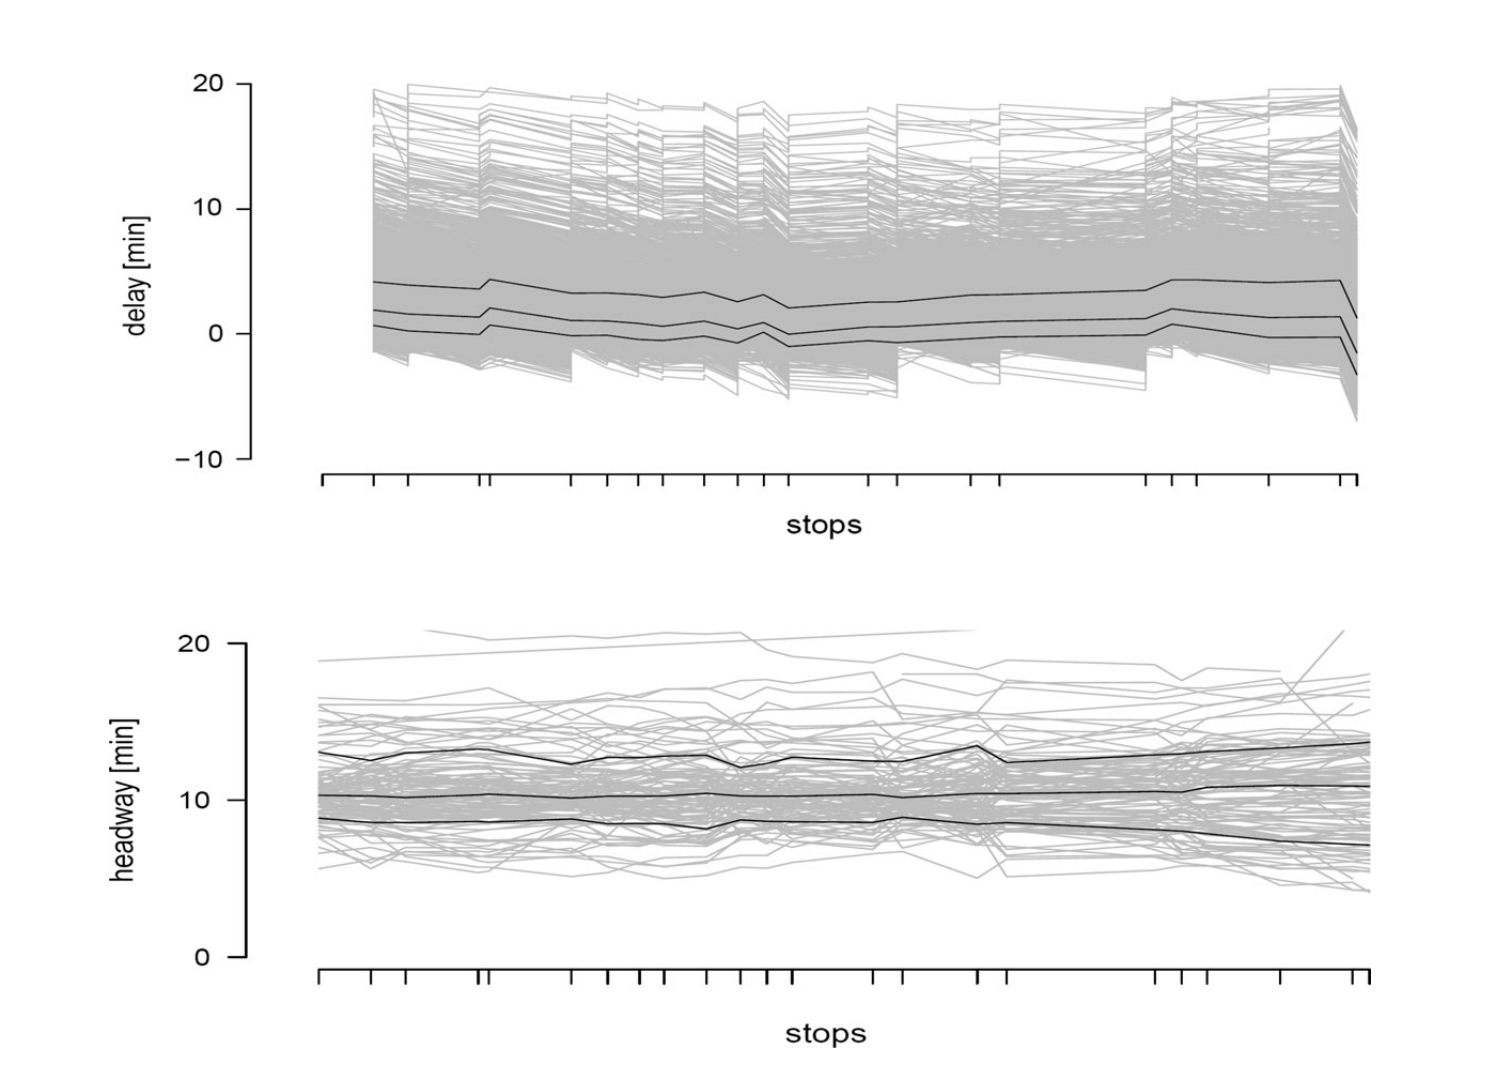
\includegraphics[width=0.8\textwidth]{van-oort-1}
	\caption{Vehicle delays (upper) and headways (lower) along a single route \autocite[378]{van-oort-2015}}
	\label{fig:van-oort-1}
\end{figure}

In \cref{fig:van-oort-2}, one can see a network-wide visualization, where each station is colored in a gradient from green to red, representing the average delay recorded at that station. It shows that overall there are only a few problem areas which are mostly series of stops where delays may accumulate. Interestingly, there are stations with a negative average delay, meaning an earlier-than-planned arrival. This effect can in certain cases be an expected result of including a leeway in schedules for important transfer hubs. If not intentional, such early arrivals can simply be solved by updating scheduled departure data \autocite[379--380]{van-oort-2015}.

\begin{figure}[h]
	\centering
	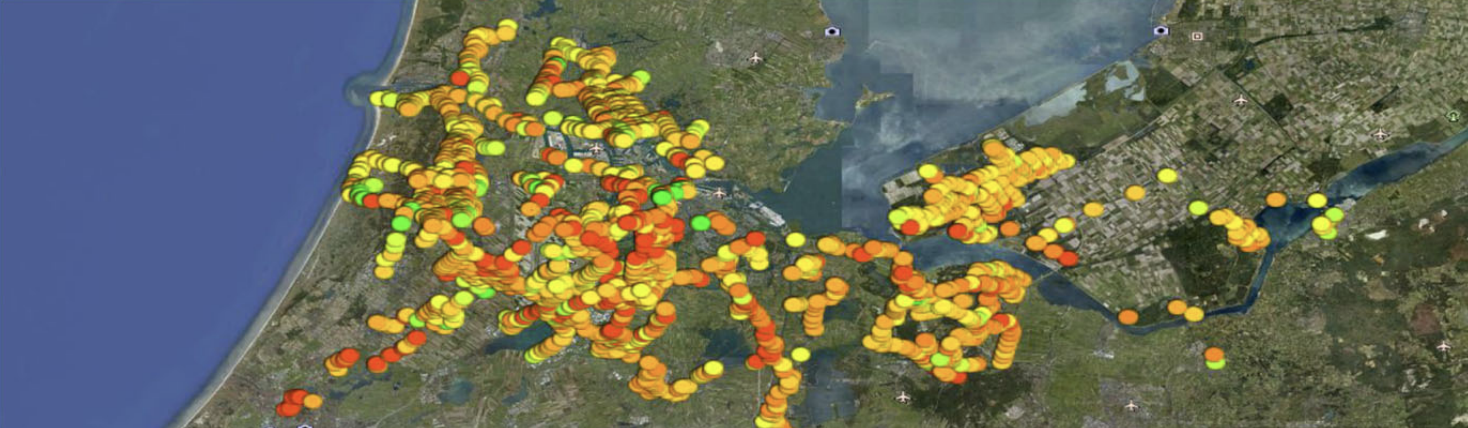
\includegraphics[width=0.9\textwidth]{van-oort-2}
	\caption{Average delay per stop (green early, yellow on time, red late) \autocite[379]{van-oort-2015}}
	\label{fig:van-oort-2}
\end{figure}

After this static analysis of historical data, the authors fitted the data to a normal distribution in order to provide passengers with so-called \textit{enriched travel advice}, where predictions based on said distribution are added to trip planning results. This information includes probabilities of delays, early departures or transfer feasibility. Additionally, they developed a tool for a more scientific analysis of collected data. This software was used on another data set from the transit network of Utrecht and was able to detect multiple bottlenecks in the network, for example, long dwell time on bus routes \autocite[380--387]{van-oort-2015}.

\subsection{Portland}

In 1993, \textcite{strathman-1993} presented a baseline study of the Portland metropolitan area transit network as part of an operations control plan implemented by the city's transit agency \textit{Tri-Met}. This plan aimed to improve the growing challenges the network was facing regarding service reliability. Like \textcite{van-oort-2015}, the authors state that for short intervals, passengers do not care about vehicles running exactly on time, but rather whether the service runs regularly and reliably. In addition to grouping causes for delays into internal and external ones, the authors divide possible countermeasures into short-term and long-term actions. Short-term actions are ones to counter unanticipated delays such as holding vehicles at a stop in case of early arrival or adding additional vehicles to a route. Long-term actions on the other hand are helpful for systemic delays which are not caused by a single unexpected event. Examples include improving driver behavior through additional training or a reward system for good on-time performance. Additionally, the schedule itself can be the root cause and a redesign with longer run times or longer layover times at the end of lines may be the solution for consistent delays. The authors also state that a more complex network with longer routes generally results in worse on-time performance than one with short routes and only a few stops. Also, lines where the highest loads occur at the first few stations are more likely to show higher delay rates. As a result, public transport providers have to balance satisfying the demands of passengers and thus network complexity with on-time performance, taking various factors such as efficient use of resources into consideration. \autocite[93--94]{strathman-1993}.

The study was conducted by manually recording arrival times on 200 trips on 59 different bus lines in the Portland metropolitan area, resulting in a total of 1552 recorded bus arrival times. Of those, 1360 or 87.6\% were punctual, with an arrival considered punctual if it falls within a range of being one minute early to five minutes late. The authors found that driver experience has a measurable effect on on-time performance, with part-time drivers being more prone to late arrivals than their full-time colleagues. Furthermore, they confirmed that early arrivals and delays occur more often during afternoon peak hours. Interestingly, they did not observe this effect for morning peak hours. In fact, arrivals were more likely to be early than late if they did not follow the schedule, indicating that planners overcompensated for morning rush hour traffic by increasing running more than necessary \autocite[97--99]{strathman-1993}.

\subsection{New York City}

A team of researchers from the Data, Research, Development (DRD) department of the New York City Transit Authority developed a tool for visualizing problem areas in New York's subway system. It detects areas where trains run slower than normal or show longer than normal intervals between trains. In addition to highlighting the results with a severity level, an interactive map display the locations of trains in real-time. This interactive map is used by the communications team in order to inform customers via social media channels about those problems occurring in the network. While there were similar tools already available for the New York transit network, these tools had significant limitations such as only allowing to view one direction of one line at a time. This required the monitoring staff to switch between the lines constantly to keep an overview. \autocite[1--3]{caspari-2021}

To gather the required train location data, the authors used a combination of real-time station arrival feeds and data provided by the signaling system. To compare running times between two stations or signaling segments, they relied on manual recordings by the transit authority rather than schedule data. They found that actual running times can deviate from scheduled ones and thus using schedules alone would result in less accurate calculations \autocite[4]{caspari-2021}. Both large intervals and slow trains are calculated and displayed on multiple levels of detail. Longer-than-normal intervals are first calculated for stops or track segments, then aggregated into bigger areas of three or more stops if applicable. For slow trains it is done similarly, ranging from single stuck trains to entire areas consisting of multiple stations where trains run significantly slower than expected. All results are then categorized into \textit{moderate}, \textit{severe} and \textit{very severe} problems, aiming to provide passengers with consistent information and suggested actions depending on the severity level \autocite[6--7]{caspari-2021}.

The interactive map that \textcite{caspari-2021} developed needed to cater to various needs, providing both an overview to detect emerging problem areas and the ability to see detailed information about a specific problem. The solution was a zoomable map, in addition to a text-based sidebar and tooltips for stations and line segments. Additional features include different available themes for severity levels, dark and light themes for the entire app and a text-only mode that displays the data in a tabular layout instead of the interactive map \autocite[8--9]{caspari-2021}. The tool was developed for more than one year and is in successful use since then. Being entirely web-based, it even allowed for easy access during the COVID-19 pandemic for the communications personnel \autocite[11]{caspari-2021}.

\subsection{Stochastic models}

Various authors have studied the fitting of delay data to statistical distribution models in order to be able to make predictions over possible future delays. \textcite{yuan-2008} found that while other distributions may provide more flexibility and adjustable parameters, a negative exponential distribution is most of the time a valid and easy-to-understand distribution to model both arrival and departure delays \autocite[173--174]{yuan-2008}. Depending on the data set and the exact delay variable being measured, other distributions might fit better. For example, \textcite[90]{goverde-2013} fitted their data of trains arriving in Utrecht to a Weibull distribution, which is a distribution that receives multiple input parameters and---depending on one of those parameters---can result in an exponential distribution too \autocite[88]{hallinan-1993}. \textcite[61]{yuan-2006} confirmed that the Weibull distribution most of the time offers the best fit. In some cases, however, other distributions such as beta, gamma or log-normal distributions model departure delays the best \autocite[61]{yuan-2006}.

\subsection{Data availability}

\subsubsection{\acf{HAFAS}}

In Germany, Austria and Switzerland but also other European countries, \acs{HAFAS}, short for \textit{\acl{HAFAS}} (HaCon Timetable-Information-System), is a popular system for retrieving timetable information as well as intermodal journey planning. It is developed by a subsidiary of Siemens and available since the late 1980s, and with that one of the first tools on the market, promising an algorithm that performs route calculation in less than six seconds. Each public transport company gets its own \ac{HAFAS} deployment, which all share common terminology and endpoints, but can however use custom configurations and feature availability. While the endpoints are usually not openly documented by the respective companies, they do not restrict access using \ac{API} tokens or similar measures and are therefore easily accessible \autocites{computerwoche-1988}{redmann-2023b}.

For this thesis, the  \ac{HAFAS} endpoint by \ac{VOR}, the transport authority of the eastern regions of Austria, was used for collecting the necessary data. While the \ac{API} itself returns data in the  \ac{HAFAS} Raw Data Format, the JavaScript library \textit{hafas-client} converts this into the much easier-to-work-with \ac{FPTF}, which is inspired by the widely used \ac{GTFS} format and uses \ac{JSON} as its serialization format \autocite{redmann-2023a}.

The library provides a multitude of endpoints, both for station and trip data. Aside from fetching information about a stop or station, the \texttt{nearby} endpoint for example can retrieve all locations that are within a given walking distance in minutes, which is especially useful for building consumer-facing public transport applications. It also includes endpoints for journey planning between two given locations. Similar to \texttt{nearby}, the \texttt{reachableFrom} endpoint returns all stations that are reachable from another station, but instead of walking distance public transport journeys are calculated. Another endpoint that provides opportunities for interesting applications is \texttt{radar}, which returns the locations of all vehicles within a given radius. While location data is not available for all vehicles, this can certainly be used as a foundation for appealing visualizations. The two most important endpoints for this thesis however are \texttt{arrivals} and \texttt{departures}, which provide accurate real-time data for one or more given station(s). In addition to planned and actual arrival/departure times, they also calculate the difference, providing the consumer with a ready-to-use delay value in seconds \autocites{redmann-2023a}{redmann-2023c}.

\subsubsection{\acf{GTFS}}

\ac{GTFS} is a format specification initially developed by Google which later---after its widespread usage in many non-Google systems---has been renamed from \textit{Google Transit Feed Specification} to \textit{General Transit Feed Specification}. It allows public transport agencies to offer their data in a unified format, understood by various consumer applications, ranging from visualization tools to trip-planning mobile applications. The core of \ac{GTFS} is a static feed of text files that contain the whole schedule and additional information about the network. The \ac{GTFS} reference document specifies five required files: \texttt{agency.txt}, \texttt{stops.txt}, \texttt{routes.txt}, \texttt{trips.txt} and \texttt{stop\_times.txt}. One can see that the structure of the data is similar to \ac{HAFAS}. Routes are a group of trips that are offered to passengers as a line or service. Arrival and departure data for those trips are then collected in \texttt{stop\_times.txt} \autocite{gtfs-2022-schedule}.

In contrast to \ac{HAFAS} however, these static files do not provide any historical or real-time data, but instead the planned schedule at the time of publishing. For real-time data, there exists a special extension to \ac{GTFS} called \ac{GTFS} Realtime. As a data format, \ac{GTFS} Realtime uses Protocol Buffers, a language-agnostic serialization format developed by Google. As real-time updates naturally come with a significantly higher level of detail than static text files, the provided data structures are entirely different. Instead of static text files, messages such as \texttt{TripUpdate}, \texttt{VehiclePosition} or \texttt{StopTimeEvent} are exchanged between the feed provider and connected clients \autocite{gtfs-2022-realtime}. 

Since 2017, the city of Vienna provides \ac{GTFS} schedule data as part of the \textit{Open Government Data} initiative. With its real-time extension, \ac{GTFS} would have been able to provide all the necessary data for this thesis, especially planned and actual departure data. However, as the \textit{hafas-client} library uses the \ac{JSON}-based \ac{FPTF} format instead of more complicated Protocol Buffers, \ac{HAFAS} was chosen as a primary data source instead of \ac{GTFS}.

\section{Implementation}
\label{sec:implementation}

In this section, after introducing Vienna's public transport network, the data collection process is described in detail. Next, the results of the delay analysis are presented, showing results both on a network-wide level and in more detail for single lines or stations. Finally, visualizations that try to make the large data set easier to understand are presented. All information about the network, especially locations of stations and lines was gathered from the network map provided by the network operator Wiener Linien \autocite{wiener-linien-2023}.

\subsection{Vienna's public transport network}

The public transport network in the city of Vienna is very popular
and well-received among the city's population. A case study by \textcite[917,921]{haslauer-2015} showed that 75 percent of the population uses the network multiple times per week and that the average satisfaction lies at 1.57 when rated on a scale from 1 to 5, with 1 being the best score (very satisfied). One factor of the high popularity is the comparatively cheap access to the system with a yearly ticket costing 365 euros, resulting in 852,300 of those tickets sold in 2019 \autocite{wiener-linien-2020}.  

The network is owned and operated by Wiener Linien, a subsidiary of Wiener Stadtwerke Holding, which in turn is fully owned by the city of Vienna.
The network consists of 5 metro lines, 28 tram lines and 131 bus lines and has a total length of 1169 kilometers \autocite{wiener-linien-2020}. Additionally, there is a suburban rail line connecting the city center with the town of Baden, operated by another subsidiary, Wiener Lokalbahnen. The line contributes 10.3 million to the total 606.1 million passengers transported by both companies in 2021 \autocite[24]{wiener-stadtwerke-2022}. Furthermore, Austria's federal railway operator ÖBB runs 10 suburban train lines from Vienna to and from neighboring towns in Lower Austria, adding another 89 million yearly passengers to Vienna's transit network \autocite{oebb-2023}.


\subsection{Data collection}

The necessary data for detecting potential delay hotspots were collected over a duration of one month, specifically from \DTMdisplaydate{2023}{2}{18}{} to \DTMdisplaydate{2023}{3}{20}{}.
The collection was done by automated scripts using the \textit{hafas-client} JavaScript library available on GitHub.\footnote{\url{https://github.com/public-transport/hafas-client} (Accessed \DTMdisplaydate{2023}{4}{30}{})} It can be used to query \ac{HAFAS} \ac{API} endpoints from various public transport companies. In the case of Vienna, the relevant company is \ac{VOR}, the transport authority for the eastern region of Austria, which includes the federal states of Vienna, Lower Austria and Burgenland. The following subsections try to explain in more detail how both station and departure data were collected and persisted for further analysis.

\subsubsection{Stations}

Departure and delay data can be queried using the \texttt{departures} method available in \textit{hafas-client}. This method expects a station object or identifier as its argument, thus a list of such station identifiers had to be created first. Since there exists no method to get a collection of all stations the network contains, the \texttt{nearby} method was used to get a list of stations within a radius (measured in meters of walking distance) from a specified coordinate pair. An example of such a query can be seen in \cref{code:stations}; a \texttt{station} object contained in the response is shown in \cref{code:station-res}. 

\begin{lstlisting}[language=JavaScript, caption={Retrieving nearby stations from given coordinates}, label={code:stations}]
import { createClient } from "hafas-client";
import { profile } from "hafas-client/p/vor/index.js";

const hafas_client = createClient(profile, "hafas-ba");

const center = {
    type: "location",
    latitude: 48.2084,
    longitude: 16.3778,
};

const locations = await hafas_client.nearby(center, {
	products: {
		tram: true,
		"u-bahn": true,
		"city-bus": true,
	},
	subStops: false,
	entrances: false,
	linesOfStops: true,
	results: 5000,
	distance: 100_000,
});
\end{lstlisting}

\begin{lstlisting}[caption={\texttt{station} object returned by the \ac{HAFAS} \ac{API}}, label={code:station-res}]
{
	"type": "station",
	"id": "490132000",
	"name": "Wien Stephansplatz",
	"location": {
		"type": "location",
		"id": "490132000",
		"latitude": 48.208133,
		"longitude": 16.371631
	},
	"products": {
		"train-and-s-bahn": false,
		"u-bahn": true,
		"tram": false,
		"city-bus": true,
	},
	"isMeta": true
}
\end{lstlisting}

The idea was to choose a point in the city center and get all available stations by using a maximum walking distance of 20,000 meters, far exceeding the theoretical maximum distance to the city borders following the fact that Vienna has a maximum north-south and east-west extension of 22.8  and 29.4 kilometers respectively \autocite[14]{stadt-wien-2022}. It was found though that the number of stations did not increase with a maximum walking distance higher than 7200 meters, capping out at 997 found stations. In order to retrieve the rest of the stations, four additional coordinate pairs were selected which cover all missing regions, especially ones near the city border. Finally, duplicated results and results that did not include the prefix \enquote{Wien} were removed, as those are situated in the neighboring state of Lower Austria which is not covered by this thesis. Using this described method, a total of 1756 stations were collected and saved to an SQLite database. From there, they can be used for the next step, querying departure and delay data from these stations.

\subsubsection{Departures}

Collecting the desired delay data was achieved by using the \texttt{departures} method of the \textit{hafas-client} library. The method receives a list of stations and returns departure objects for those stations, which can be seen in \cref{code:departures} and \cref{code:departures-res}. These objects contain properties for planned and actual departure times and with that the resulting delay, if applicable. 

\begin{lstlisting}[language=JavaScript, caption={Retrieving departures from a given station ID}, label={code:departures}]
import { createClient } from "hafas-client";
import { profile } from "hafas-client/p/vor/index.js";

const hafas_client = createClient(profile, "hafas-ba");
const station_id = "490132000"; // Wien Stephansplatz

const { departures } = await hafas_client.departures(station_id, {
	duration: 50,
	subStops: false,
	entrances: false,
	results: 60,
});
\end{lstlisting}

\begin{lstlisting}[caption={A \texttt{departure} object returned by the \ac{HAFAS} \ac{API}}, label={code:departures-res}]
	{
		"tripId": "2|#VN#1#ST#1680820733#PI#0#ZI#66304#TA#1#DA...",
		"stop": {...},
		"when": "2023-04-07T09:33:00+02:00",
		"plannedWhen": "2023-04-07T09:32:00+02:00",
		"delay": 60,
		"platform": "2",
		"plannedPlatform": "2",
		"prognosisType": "prognosed",
		"direction": "Wien Alaudagasse",
		"provenance": null,
		"line": {
			"type": "line",
			"id": "vor-21-u1-j23-3",
			"fahrtNr": "586",
			"name": "U1",
			"public": true,
			"adminCode": "v04WL_",
			"mode": "train",
			"product": "u-bahn",
			"operator": {
				"type": "operator",
				"id": "wiener-linien",
				"name": "Wiener Linien"
			}
		},
		"remarks": [
			{ "type": "hint", "code": "LF", "text": "Niederflurfahrzeug" }
		],
		"origin": null,
		"destination": {
			"type": "stop",
			"id": "490001409",
			"name": "Wien Alaudagasse",
			"location": {...},
			"products": {...},
			"station": {...}
		},
		"currentTripPosition": {
			"type": "location",
			"latitude": 48.213994,
			"longitude": 16.383191
		}
	}
\end{lstlisting}

Since the \ac{HAFAS} \ac{API} did not reliably work when fetching departures for all 1756 stations, an alternative strategy was chosen. Instead, only one station at a time was queried in a one-second interval, specifying a time span of 50 minutes of upcoming departures included in the result. After every station was visited, the cycle starts from the beginning, which results in each station being visited approximately every 30 minutes. A unique ID consisting of the identifiers of both the trip and station was assigned to each departure result in order to detect results that were already included in previous cycles. In those cases of duplicates, the newer result was selected in order to ensure the most current and accurate data was saved for each departure. The source code for this process can be seen in \cref{code:monitor}. This script was then executed with \texttt{nohup} so that it can continuously run in the background on a Linux server during the collection period.

\begin{lstlisting}[caption={A \texttt{departure} object returned by the \ac{HAFAS} \ac{API}}, label={code:monitor}]
import { hafas_client } from "./client.js";
import { db } from "./db.js";
import { sleep } from "./utils.js";

const station_ids = await db.selectFrom("stations").select("id").execute();
let i = 0;

while (i < station_ids.length) {
	const { id: station_id } = station_ids[i];
	const { departures } = await hafas_client.departures(station_id, {
		duration: 50,
		subStops: false,
		entrances: false,
		results: 60,
	});
	let inserted = 0;

	for (const dep of departures) {
		const new_dep = {
			id: "",
			direction: dep.direction,
			delay: dep.delay,
			when: dep.when,
			planned_when: dep.plannedWhen,
			station_id: dep.stop?.station?.id ?? dep.stop?.id,
			station_name: dep.stop?.station?.name ?? dep.stop?.name,
			line_id: dep.line?.id,
			line_name: dep.line?.name,
			product: dep.line?.product,
		};
		new_dep.id = `${new_dep.station_id}_${dep.tripId}`;
		const result = await db
			.insertInto("departures")
			.values(new_dep)
			.onConflict((oc) => oc.column("id").doUpdateSet(new_dep))
			.execute();
		inserted += +result[0].numInsertedOrUpdatedRows ?? 0;
	}

	await sleep(1000);
	i++;

	if (i === stations.length) {
		i = 0;
	}
}
\end{lstlisting}

\subsubsection{Persisting the collected data}
\label{sec:persisting}

For persisting the collected data, SQLite, a self-contained \ac{RDBMS} was used together with the TypeScript based \textit{kysely} library for building \ac{SQL} queries. Using a \ac{RDBMS} with a query builder has the advantage of providing a great developer experience, with type-safe methods for querying the database and features like insertion conflict handling, which was especially important for assuring no duplicate stations and departures were saved.

While a \ac{RDBMS} like SQLite is a good tool for data collection, the resulting departures table was converted into a \ac{CSV} file for further persistence and analysis. One reason for that is the substantially smaller file size of 4.6\,GB, compared to the SQLite file's size of 8.2\,GB, resulting in a reduction of around 44\%. The collected data set contains a total of 13,720,298 recorded departures with an average of 457,347 departures per day.
\subsection{Delay analysis}
\label{sec:analysis}

\subsubsection{Filtering irrelevant data}

Since the main focus of this thesis is to analyze the public transport network of Vienna, long-distance train services were stripped of the resulting data set. Since the \ac{API} endpoint does not differentiate between long-distance trains and suburban regional trains, the latter also were removed in this step. This means that in the following analysis, only public transport products by Wiener Linien, which includes metros, trams and buses, are considered. Long-distance trains have widely different characteristics in comparison to high-frequent inner-city transport methods such as trams or buses. These differences were quickly visible when conducting the first screening of the collected data. The most delayed trips were all Railjet (Austrian high-speed train service) services from neighboring countries, with delays in the multiple-hour range. While an interesting observation, these types of delays are not the intended research area of this thesis, which instead lays its focus on those inner city lines mentioned above. Additionally, the hybrid tram/train line \textit{Badner Bahn} also had to be excluded from further analysis since the collected data did only include scheduled timetable departures and not real-time departure times. This means that for this particular line, no delay data could be collected.

\subsubsection{Tools and technologies}

As mentioned in \cref{sec:persisting}, the resulting SQLite file was converted into a \ac{CSV} file for easier organization and handling. The following results were all gathered by utilizing the widely used data analysis library \textit{pandas} for Python. Visualizations on the resulting data frames were then produced by \textit{plotly}, another Python library commonly used for visualization and charting tasks. The most common figures such as line charts, bar charts, box plots or scatter plots are all available through the \textit{plotly-express} subpackage, which was used for all following visualizations. For figures including a map, the underlying map data is provided by \textit{Mapbox}.

\subsubsection{Basic summary}

To gather an initial overview of the collected data, we first want to highlight a few general characteristics of the data set. \Cref{table:basics} shows the basics statistical data points of the \texttt{delay} measurements. One can see that the mean delay was 14.68 seconds, with a minimum of -3600, meaning a one-hour early departure, and a maximum delay of 10,920 seconds, or approximately 3 hours. The high standard deviation of 115.62 seconds indicates that the data points are highly spread out around the mean. It is therefore unsurprising that the \nth{25}, \nth{50} and \nth{75} percentile are all 0 since actual punctuality rates of public transport networks mostly lay between 90 and 99 percent, for example with national rail services in Vienna having punctuality rates of around 96\% \autocite{oebb-2023b}. In fact, \cref{table:punctuality} shows that 12\% of the recorded departures had a delay greater than zero. However, the definition of punctuality varies from company to company and rates are usually calculated with a specified maximum delay threshold of one to five minutes \autocite[723]{chen-2009}. With a maximum delay of one minute, the punctuality rate falls at 94.17\%, while a maximum of five minutes results in 99.25\% punctuality. For all further punctuality rate calculations, we assume a departure is punctual if it has a maximum delay of three minutes or less.

\begin{table}
	\centering
	\begin{tabular}{lr}
		\toprule
		count &  13,720,398 \\
		mean  &  14.68 \\
		std   &  115.62 \\
		min   & -3600 \\
		25\%   &  0 \\
		50\%   &  0 \\
		75\%   &  0 \\
		max   &  10,920 \\
		\bottomrule
	\end{tabular}
	\caption{Basic summary of \texttt{delay} column}
	\label{table:basics}
\end{table}

\begin{table}
	\centering
	\begin{tabular}{rr}
		\toprule
		Delay threshold [min] & Punctuality rate \\
		\midrule
		0 &  0.8791 \\
		1  &  0.9417 \\
		2   &  0.9704 \\
		3   & 0.9837 \\
		4   & 0.9895 \\
		5   &  0.9925 \\
		\bottomrule
	\end{tabular}
	\caption{Punctuality rates depending on minimum delay}
	\label{table:punctuality}
\end{table}

\subsubsection{Most and least delayed lines}

When grouping all departures by line and sorting by punctuality rate, it shows that the most punctual lines are all bus lines, as shown in \cref{table:overall-top10-most}. Also, the nine most punctual lines all have perfect punctuality rates of 100\%, the first line with a rate less than 100\% is bus 54B with 99.98\%, landing in tenth place. Six of those lines with 100\% punctual departures even have a mean delay of 6 seconds or less, meaning only very few or no delays were recorded. Line N62 is the first one with a higher mean delay of 22.17 seconds, but still a perfect punctuality rate of 100\%. When looking at lines with the lowest punctuality rate in \cref{table:overall-top5-least}, one can see that again buses dominate and only one tram line appears as the fifth least punctual line, namely tram 71 with a punctuality rate of 95.51\% and a mean delay of 24.87 seconds. Line 42A has the lowest punctuality rate and also by far the highest mean delay with 149.01 seconds, while the other three bus lines show mean delays between 30.05 and 51.89 seconds.

\begin{table}
	\centering
	\begin{tabular}{llrr}
		\toprule
		Line & Product & Punctuality rate & Mean delay [s] \\
		\midrule
		ZF & Bus &  1.0 & 0.00 \\
		73A & Bus &  1.0 & 0.00 \\
		34A & Bus &  1.0 & 0.00 \\
		U6E & Metro/bus &  1.0 & 0.00 \\
		N29 & Bus &  1.0 & 0.97 \\
		N66 & Bus &  1.0 & 1.54 \\
		2A & Bus & 1.0 & 1.69 \\
		N46 & Bus &  1.0 & 5.99 \\
		N62 & Bus & 1.0 & 22.17 \\
		54B & Bus &  0.9998 & 4.56 \\
		\bottomrule
	\end{tabular}
	\caption{Top ten most punctual lines}
	\label{table:overall-top10-most}
\end{table}

\begin{table}
	\centering
	\begin{tabular}{llrr}
		\toprule
		Line & Product & Punctuality rate & Mean delay [s] \\
		\midrule
		42A & Bus & 0.9030 & 149.01 \\
		10A & Bus &  0.9245 & 51.89 \\
		63A & Bus &  0.9505 & 30.05 \\
		95A & Bus & 0.9527 & 39.14 \\
		71 & Tram &  0.9551 & 24.87 \\
		\bottomrule
	\end{tabular}
	\caption{Top five least punctual lines}
	\label{table:overall-top5-least}
\end{table}

Because of the dominance of bus lines, a further differentiation between bus, tram and metro lines may be of interest. \Cref{table:metro-top5} shows the city's five metro lines ordered by their punctuality rate. Line U6E is a special case as it is categorized as a metro line while it actually operated as a bus and acted as a replacement for a few stops on line U6 during one weekend of construction work. All other, actual metro lines show quite high punctuality rates too, with U2 being the least punctual line which still had 98.65\% punctual departures. Line U6 is the most punctual line, showing a punctuality rate of 99.5\%. Mean delays generally increase for lower punctuality rates, though remain at a low level with values between 7.89 and 18.52 seconds.

\begin{table}
	\centering
	\begin{tabular}{lrr}
		\toprule
		Line & Punctuality rate & Mean delay [s] \\
		\midrule
		U6E & 1.0 & 0.00 \\
		U6 &   0.9950 & 10.14 \\
		U1 &   0.9944 & 7.89 \\
		U3 &   0.9926 & 12.11 \\
		U4 &   0.9882 & 14.95 \\
		U2 &   0.9865 & 18.52 \\
		\bottomrule
	\end{tabular}
	\caption{Metro lines by punctuality rate}
	\label{table:metro-top5}
\end{table}

\Cref{table:tram-top5-most} and \cref{table:tram-top5-least} show only tram lines, with line 52 showing the highest punctuality rate of 99.77\% and line 71 the lowest with 95.51\%. Similar to U6E, U2Z is a replacement line during construction work. However, in daily operation, it is treated like a regular tram line, as it is planned to be in service for more than two years \autocite{stadt-wien-2021}. For the most punctual trams, mean delays show very low values, with three out of the top five having negative values ranging as low as -32.24 seconds for line U2Z. The least punctual trams lines have mean delays of around 30 seconds, only line 1 has a lower value of 10.88 seconds.


\begin{table}
	\centering
	\begin{tabular}{lrr}
		\toprule
		Line & Punctuality rate & Mean delay [s] \\
		\midrule
		52 &  0.9977 & 4.22 \\
		U2Z &  0.9955 & -32.24 \\
		33 &   0.9954 & -15.99 \\
		37 &   0.9929 & 10.53 \\
		30 &   0.9928 & -2.41 \\
		\bottomrule
	\end{tabular}
	\caption{Top five most punctual tram lines}
	\label{table:tram-top5-most}
\end{table}

\begin{table}
	\centering
	\begin{tabular}{lrr}
		\toprule
		Line & Punctuality rate & Mean delay [s] \\
		\midrule
		71 &  0.9551 & 24.87 \\
		2 &   0.9554 & 26.62 \\
		1 &   0.9678 & 10.88 \\
		D &   0.9727 & 32.49 \\
		O &   0.9737 & 23.80 \\
		\bottomrule
	\end{tabular}
	\caption{Top five least punctual tram lines}
	\label{table:tram-top5-least}
\end{table}

\subsubsection{Most and least delayed stations}

Following the fact that entire lines showed punctuality rates of 100\%, all stations that serve these lines (but not others), also have a punctuality rate of 100\%. More interesting are the stations with the lowest rates of punctual departures, shown in \cref{table:stations-least-10}. They are all bus stops again, interestingly however the very least punctual stop, \textit{Blaasstraße}, has a difference in punctuality rate to the next one (i.e. second least punctual) of almost eight percentage points while the maximum difference of all other neighboring punctuality rates in fact lies at 0.87 percentage points. Also, while mean delay values are generally high for the least punctual stations, they do not strictly increase with lower punctuality rates. \textit{Krenngasse}, for example, has the fifth-highest mean delay but ranks tenth for punctuality rate. \Cref{fig:boxplot-stations} shows box plots of the stations' delays with stations grouped by their available products. In these plots, \textit{Blaasstraße} is clearly visible on the very left of the plot for bus stations and overall, indicating it is an outlier.

Again, since most and least delayed stations are all bus stations and to get more results about highly frequented stations that are relevant to more passengers, \cref{table:metro-stations-top5-most} shows only the highest-ranked stations that serve at least one metro line, while \cref{table:metro-stations-top5-least} shows the five least punctual metro stations in the network. Of those stations, \textit{Neue Donau} is the most punctual with a punctuality rate of 99.9\%, while \textit{Aspern Nord} shows the most delays with its punctuality rate being 97.11\%. The five most punctual stations show low mean delays between 2.73 and 10.71 seconds while the least punctual metro stations still have mean delays of around 20 seconds, only five seconds higher than the average of the whole data set. Three out of the five stations with the lowest punctuality rates serve metro, tram and bus lines, while all of the five most punctual stations have metro and bus services only.

\begin{figure}[h]
	\centering
	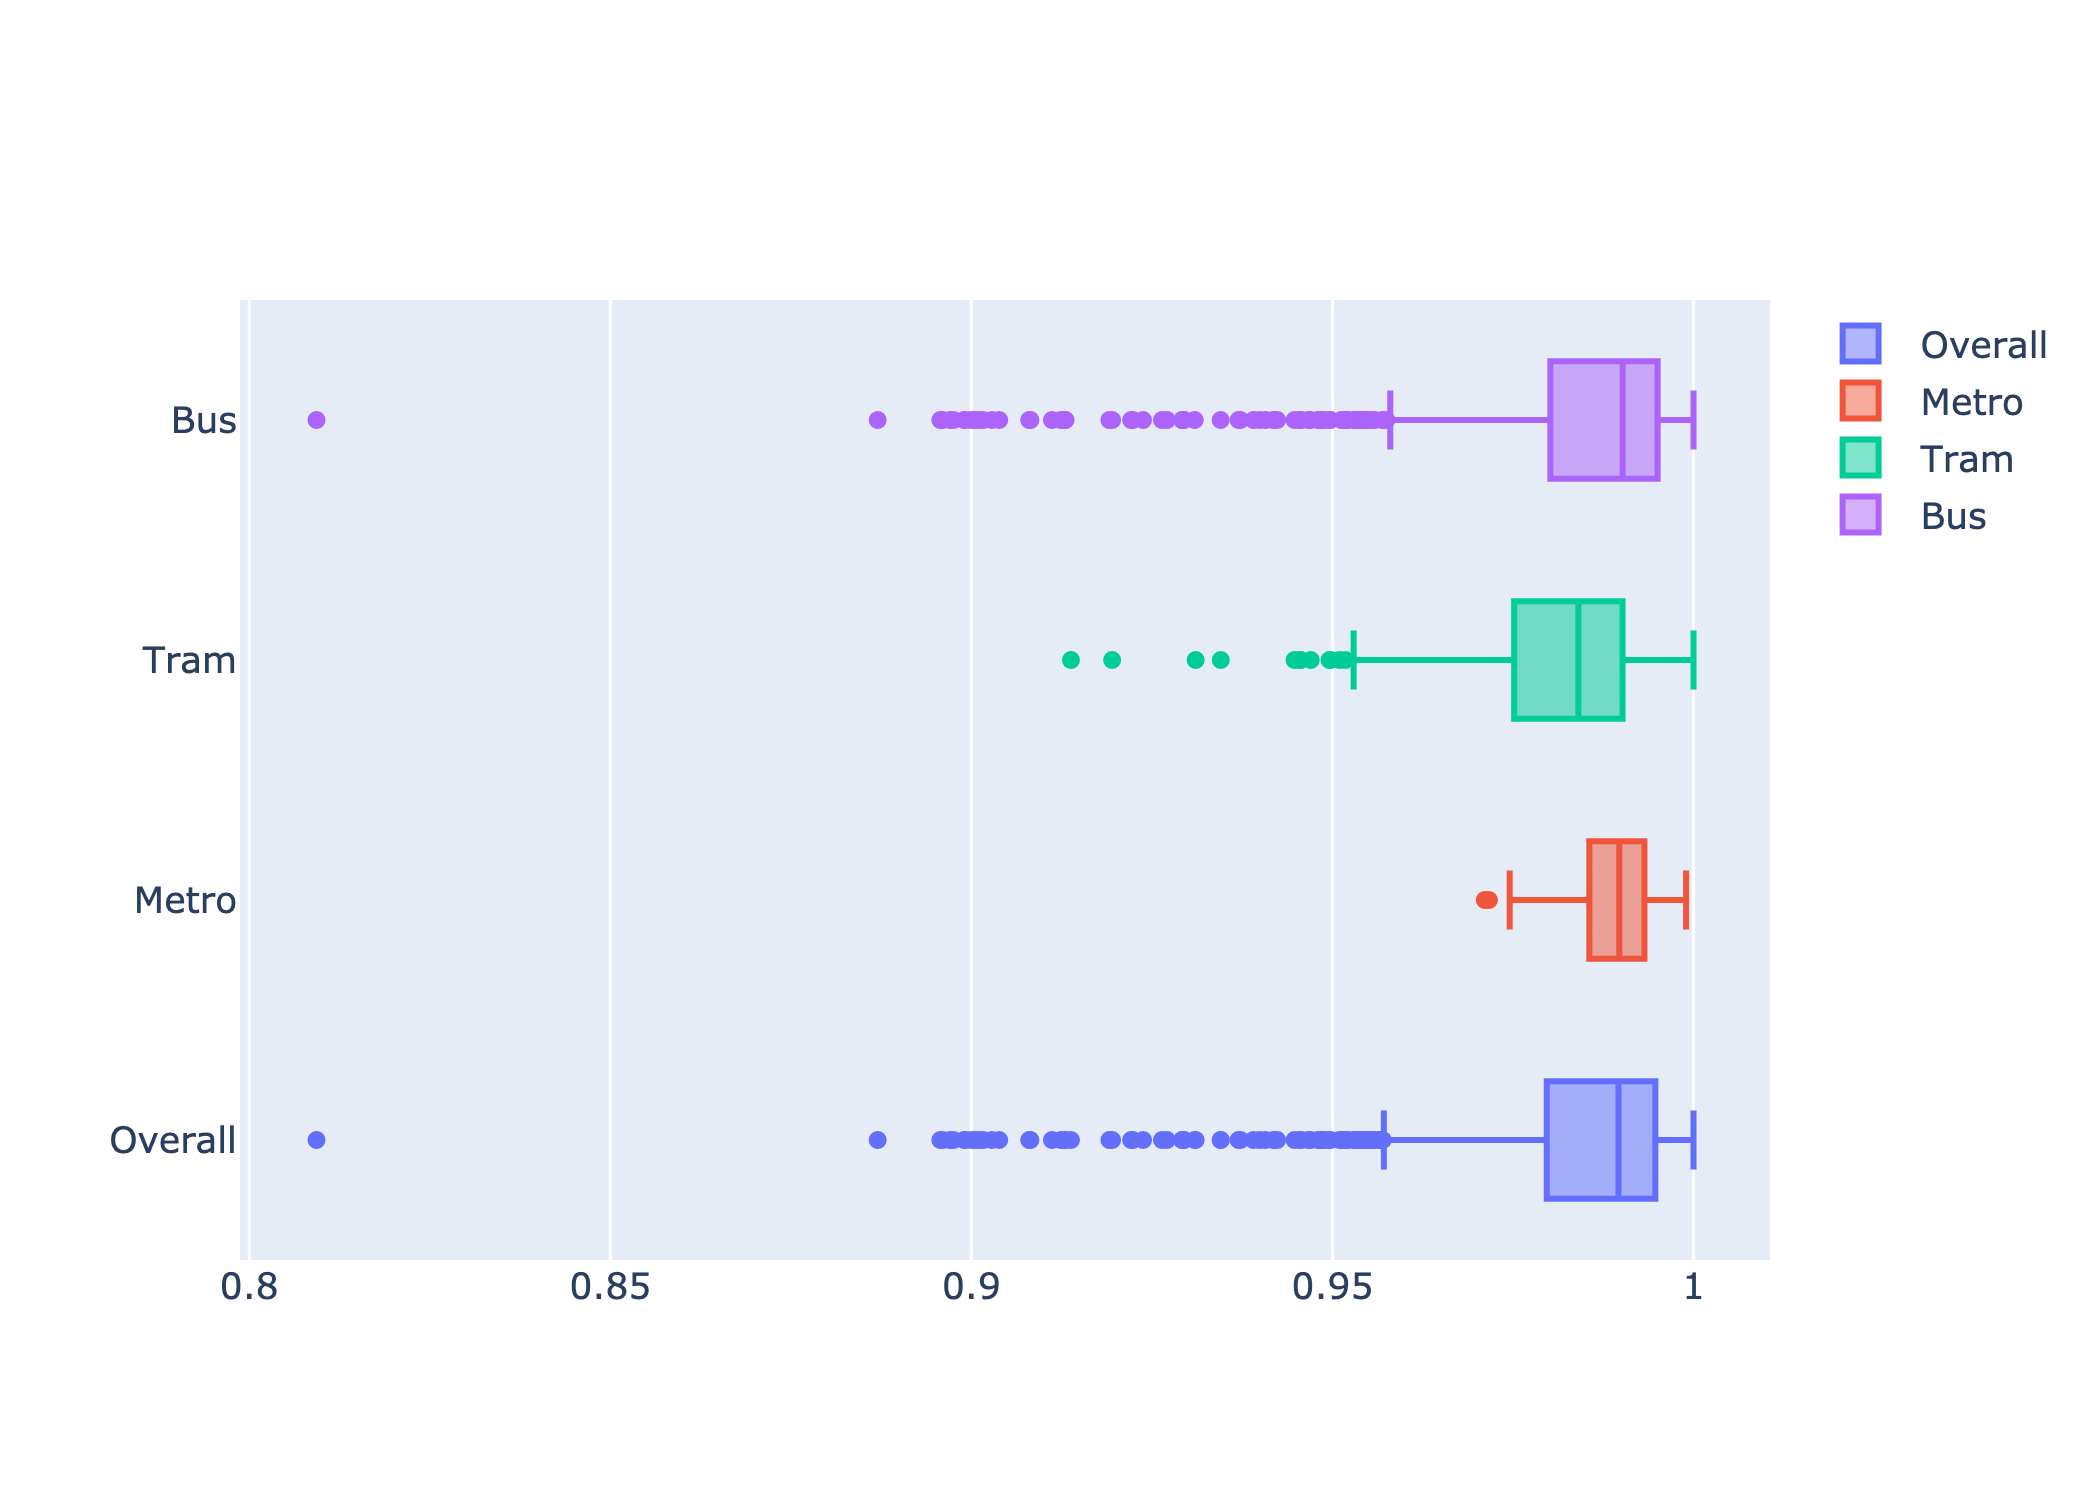
\includegraphics[width=0.9\textwidth]{boxplot-stations}
	\caption{Box plots of delay rates grouped by station type}
	\label{fig:boxplot-stations}
\end{figure}

\begin{table}
	\centering
	\begin{tabular}{llrr}
		\toprule
		Station & Products & Punctuality rate & Mean delay [s] \\
		\midrule
		Blaasstraße & Bus & 0.8093 & 115.53 \\
		Schafbergbad & Bus &  0.8870 & 178.62 \\
		Schafberg/Werfelstraße & Bus &  0.8957 & 164.45 \\
		Twarochgasse & Bus &   0.8961 & 164.66 \\
		Minciostraße & Bus &   0.8971 & 83.30 \\
		Ulanenweg & Bus &   0.8975 & 62.63 \\
		Kieslerweg & Bus &   0.8990 & 67.12 \\
		KGV Alsrückenweg & Bus &   0.8991 & 155.32 \\
		Korbweidenweg & Bus &   0.9000 & 70.19 \\
		Krenngasse & Bus &   0.9005 & 153.04 \\
		\bottomrule
	\end{tabular}
	\caption{Top ten least punctual stations}
	\label{table:stations-least-10}
\end{table}


\begin{table}
	\centering
	\begin{tabular}{llrr}
		\toprule
		Station & Products & Punctuality rate & Mean delay [s] \\
		\midrule
		Neue Donau & Metro, bus & 0.9990 & 2.73 \\
		Siebenhirten & Metro, bus &  0.9988 & 5.17 \\
		Hütteldorf & Metro, bus  & 0.9987 & 3.47 \\
		Seestadt & Metro, bus & 0.9984 & 10.71 \\
		Nestroyplatz &  Metro, bus  & 0.9966 & 6.28 \\
		\bottomrule
	\end{tabular}
	\caption{Top five most punctual stations serving metro lines}
	\label{table:metro-stations-top5-most}
\end{table}

\begin{table}
	\centering
	\begin{tabular}{llrr}
		\toprule
		Station & Products & Punctuality rate & Mean delay [s] \\
		\midrule
		Aspern Nord & Metro, bus & 0.9711 & 21.36 \\
		Taborstraße & Metro, tram, bus &  0.9717 & 21.40\\
		Johnstraße & Metro, tram, bus & 0.9746 & 23.66 \\
		Meidling Hauptstraße & Metro, bus & 0.9785 & 17.75 \\
		Schwedenplatz &  Metro, tram, bus & 0.9789 & 15.21 \\
		\bottomrule
	\end{tabular}
	\caption{Top five least punctual stations serving metro lines}
	\label{table:metro-stations-top5-least}
\end{table}

\subsubsection{Tram line 71}
\label{sec:line-71-analysis}

In previous sections, all lines or stations of the network were considered. In this section, we want to analyze and focus on one specific line. For this, tram line 71 was chosen for three reasons: Firstly, it is a highly frequented line with intervals of 7-8 minutes on weekdays and therefore much departure data was collected and is available for analysis. Secondly, it is a radial line, starting in the city center and terminating in an outer district. This type of line represents the majority of tram lines in the network. Finally, it is the tram line with the lowest punctuality rate, promising interesting results for delay measures along the line. 

\Cref{table:tram-71-stations} shows all 32 stations on line 71 sorted by their respective punctuality rate. Additionally, the mean delay was calculated for each station. The most punctual station is \textit{Kasierebersdorf, Zinnergasse} which shows a punctuality rate of 99.59\% and a mean delay of -25.15 seconds. All other stations have positive mean delays with values ranging between 18.35 and 33.63 seconds. The least punctual station, \textit{Valiergasse}, has a punctuality rate of 92.30\% and said mean delay of 33.63 seconds. Additionally, one can see that the mean delay generally increases with a lower ranking and thus lower punctuality rate. However, certain stations do not follow this pattern and show a higher mean delay than the next station down the list. For example, \textit{Ring/Volkstheater U} has with 20.42 seconds a notably higher mean delay value than the next less punctual station, \textit{Am Heumarkt}, which has a mean delay of 18.71 seconds. The same behavior can be observed for \textit{Oper/Karlsplatz U} and its neighbor in the table \textit{Unteres Belvedere}.

\begin{table}
	\centering
	\begin{tabular}{lrr}
		\toprule
		Station & Punctuality rate & Mean delay [s] \\
		\midrule
		Kaiserebersdorf, Zinnergasse &    0.9959 & -25.15 \\
		Rathausplatz/Burgtheater     &    0.9796 &  18.35 \\
		Parlament                    &    0.9788 &  18.48 \\
		Burgring                     &    0.9785 &  19.35 \\
		Börse                        &    0.9784 &  18.83 \\
		Ring/Volkstheater U          &    0.9769 &  20.42 \\
		Am Heumarkt                  &    0.9757 &  18.71 \\
		Schottentor                  &    0.9747 &  22.08 \\
		Schwarzenbergplatz           &    0.9736 &  20.88 \\
		Oper/Karlsplatz U            &    0.9734 &  23.77 \\
		Unteres Belvedere            &    0.9699 &  21.18 \\
		Rennweg                      &    0.9697 &  22.10 \\
		Kleistgasse                  &    0.9679 &  20.34 \\
		Oberzellergasse              &    0.9666 &  20.40 \\
		St. Marx                     &    0.9654 &  22.72 \\
		Litfaßstraße                 &    0.9566 &  25.04 \\
		Molitorgasse                 &    0.9554 &  25.76 \\
		Zippererstraße               &    0.9545 &  25.12 \\
		Hauffgasse                   &    0.9526 &  26.26 \\
		Enkplatz                     &    0.9459 &  29.50 \\
		Simmering                    &    0.9444 &  30.23 \\
		Braunhubergasse              &    0.9441 &  29.26 \\
		Fickeysstraße                &    0.9424 &  29.95 \\
		Weißenböckstraße             &    0.9414 &  29.48 \\
		Zentralfriedhof 1.Tor        &    0.9393 &  29.49 \\
		Zentralfriedhof 2.Tor        &    0.9369 &  30.57 \\
		Zentralfriedhof 3.Tor        &    0.9337 &  31.50 \\
		Pantucekgasse/Widholzgasse   &    0.9334 &  30.75 \\
		Zentralfriedhof 4.Tor        &    0.9329 &  30.89 \\
		Leberberg                    &    0.9322 &  30.87 \\
		Svetelskystraße              &    0.9288 &  31.78 \\
		Valiergasse                  &    0.9230 &  33.63 \\
		\bottomrule
	\end{tabular}
	\caption{Stations on line 71 sorted by punctuality rate}
	\label{table:tram-71-stations}
\end{table}

\subsubsection{Station \textit{Karlsplatz}}

\begin{table}
	\centering
	\begin{tabular}{llrr}
		\toprule
		Line & Product & Punctuality rate & Mean delay [s] \\
		\midrule
		2A & Bus & 0.9970 & 3.75 \\
		U2Z & Tram & 0.9965 & -16.20 \\
		U1 & Metro & 0.9948 & 8.29 \\
		4A & Bus & 0.9889 & 12.69 \\
		59A & Bus & 0.9854 & 18.83 \\
		U4 & Metro & 0.9811 & 17.84 \\
		71 & Tram & 0.9734 & 23.77 \\
		1 & Tram & 0.9724 & 0.76 \\
		D & Tram & 0.9721 & 37.09 \\
		62 & Tram & 0.9702 & 30.18 \\
		2 & Tram & 0.9567 & 29.59 \\
		\bottomrule
	\end{tabular}
	\caption{Lines at \textit{Karlsplatz} sorted by punctuality rate}
	\label{table:karlsplatz-lines}
\end{table}

Like \cref{sec:line-71-analysis} did for one line, this section focuses on the analysis of one station. For this, the station \textit{Karlsplatz} was chosen, as it is one of the main transfer hubs in the network. It serves two metro lines, six tram lines and three bus lines. When construction finishes in the fall of 2023, the station's third metro line U2 will continue its service to \textit{Karlsplatz}. In the meantime, tram U2Z serves as a replacement line, with one of its terminal stations located at \textit{Karlsplatz}.

In \cref{table:karlsplatz-lines}, departures at \textit{Karlsplatz} are grouped by lines and again sorted by their respective punctuality rate. Line 2A, one of the inner city buses has the best punctuality rate with 99.70\% punctual departures, together with a mean delay of 3.75 seconds. Next is U2Z, the replacement tram line for U2, showing a punctuality rate of 99.65\% and, notably, a mean delay of -16.20 seconds. Metro lines U1 and U4 show considerably lower mean delays than tram lines, with U1 having a rather low value of just 8.29 seconds and a punctuality rate of 99.48\%. Interestingly, tram lines 71, D, 62 and 2 all have similar mean delays of approximately 30 seconds. Line 1 however has a mean delay of only 0.76 seconds, even though its punctuality rate of 97.24\% is similar to the other mentioned lines. The line with the least number of punctual departures is tram line 2 with its punctuality rate of 95.67\% and mean delay of 29.59 seconds.
\subsection{Visualizations}
\label{sec:visualization}

In \cref{sec:analysis} we explored the available data and made interesting observations by looking at the numbers themselves and comparing them in a simple tabular form or with basic box plot diagrams. While this provided good insights, we as humans tend to comprehend visualizations better than raw numbers, especially for huge data sets with millions of entries such as the one on hand \autocite[2]{ware-2019}. Therefore, the following section presents and discussed some visualizations which aim to show the collected delay data in a way that is easy to understand while still providing the reader with valuable information. Specifically, the first visualizations show colored dots on a map of Vienna, with the colors representing the delay rates of those stations. Next, we present line graphs showing the variation in punctuality rate and number of departures throughout the day, separated by weekdays and weekends.

\subsubsection{Stations colored by punctuality rate}

\begin{figure}[h]
	\centering
	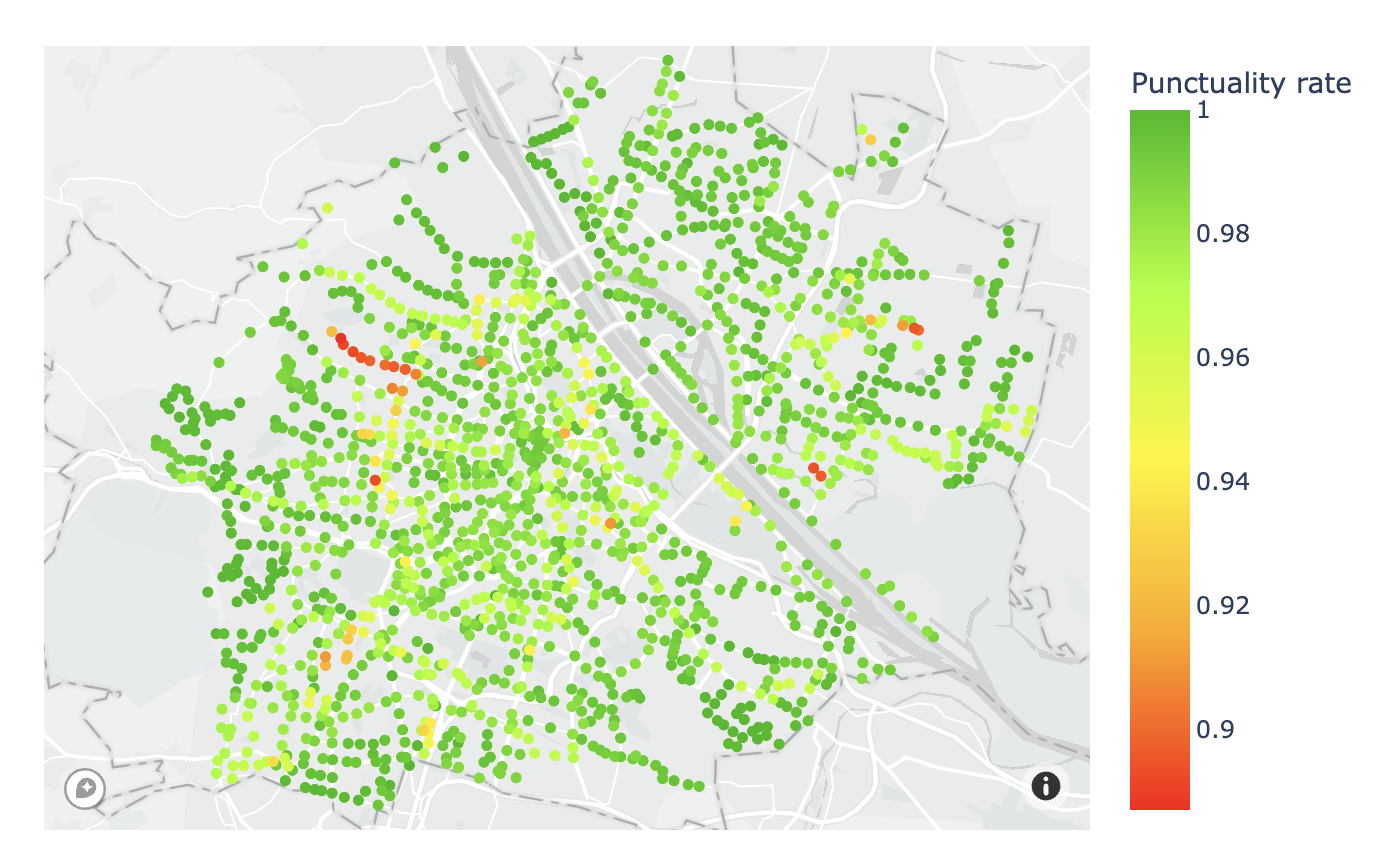
\includegraphics[width=1\textwidth]{overall-no-blaasstr}
	\caption{All stations colored by punctuality rate}
	\label{fig:overall-stations}
\end{figure}

For the first visualization, depicted in \cref{fig:overall-stations}, all stations of the network were marked with a dot at their respective location on a map of Vienna. Then, stations were colored based on their individual punctuality rate, ranging from green for a rate of 100\% to red representing a rate of 88.7\%. Since the station \textit{Blaasstraße} was already detected as an outlier in \cref{sec:analysis}, it is not included in this map as it would shift all other stations relatively far up on the color scale, resulting in an all-green map. At first glance, one can see a very good overall state, with a vast majority of stations colored light to dark green. Besides a few red spots, there is a noticeable sequence of orange and red stations, located in the northwest of the city center which all belong to bus line 42A. Besides these more delayed areas, the darkest green and thus most punctual sequences of stations can be seen on the edges of the network, most notably in the west and south of the city, in addition to the area east of the Danube River.

\begin{figure}[h]
	\centering
	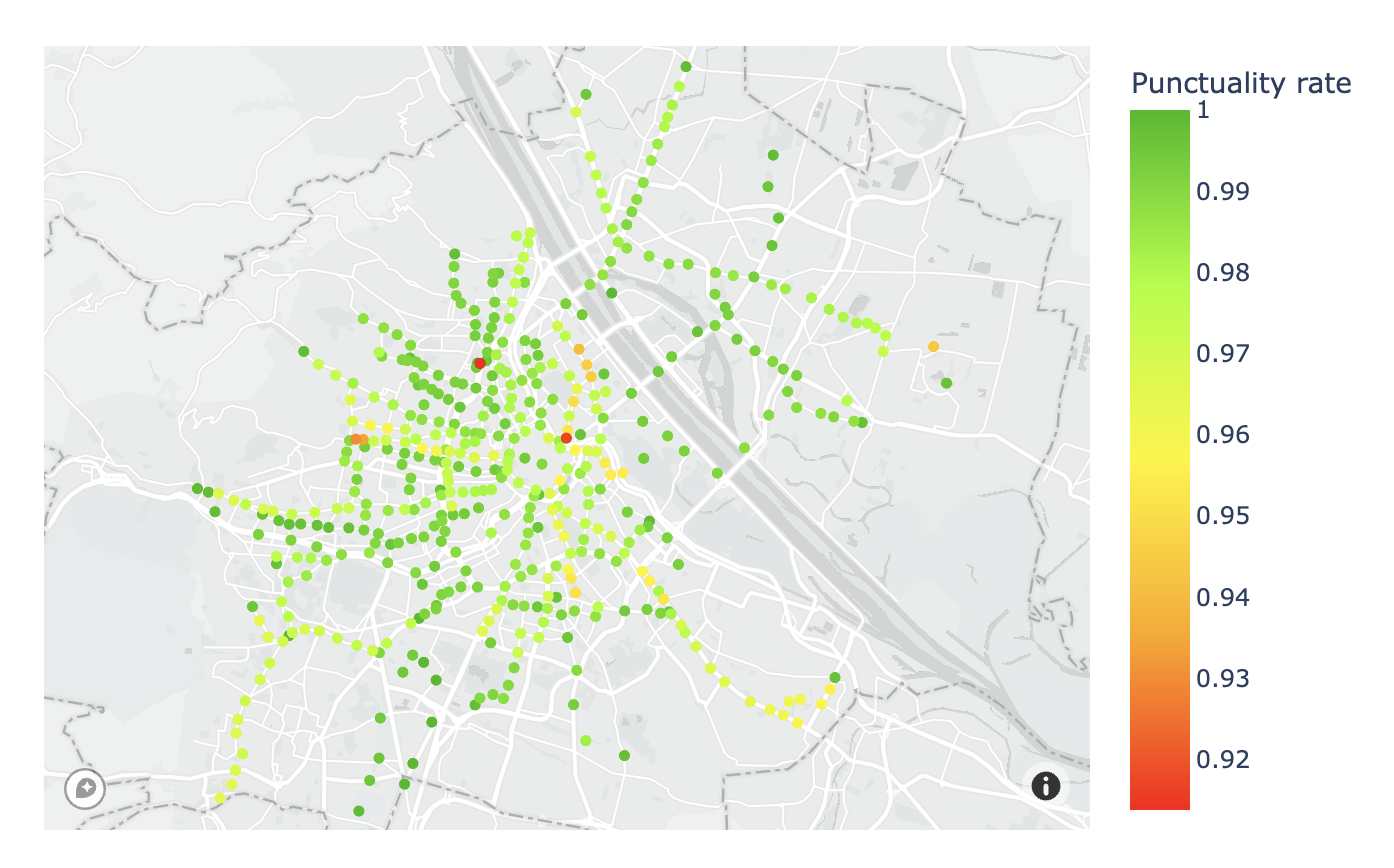
\includegraphics[width=1\textwidth]{no-buses}
	\caption{Metro and tram stations colored by punctuality rate}
	\label{fig:no-buses-stations}
\end{figure}

\begin{figure}[h]
	\centering
	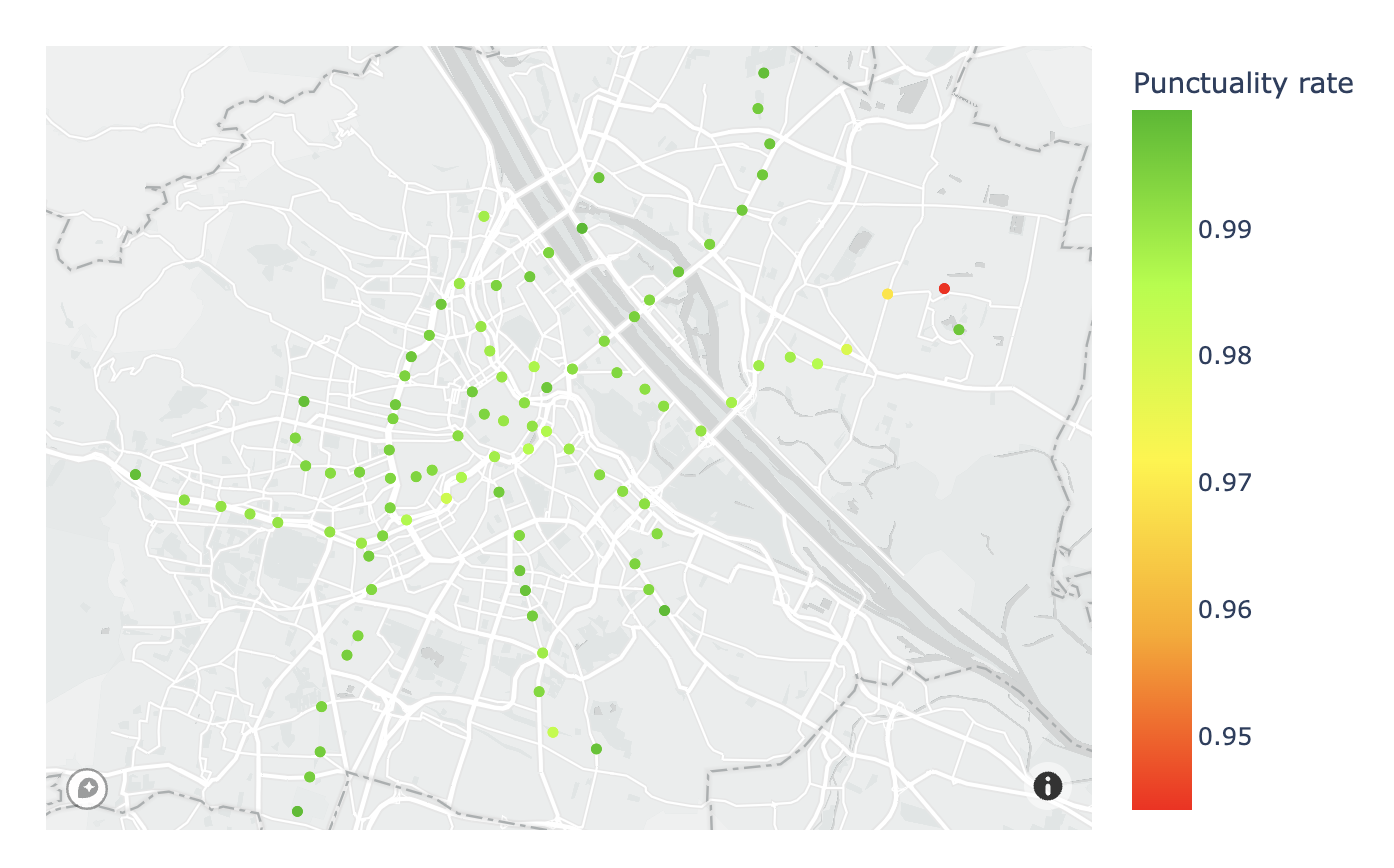
\includegraphics[width=1\textwidth]{metro-only}
	\caption{Metro stations colored by punctuality rate}
	\label{fig:metro-only-stations}
\end{figure}

Since the previous map with all bus, tram and metro stations is rather dense, \cref{fig:no-buses-stations} shows only tram and metro stations. On there, one can see two red dots, which are the stations \textit{Marsanogasse} located north of the city center and \textit{Gredlerstraße} which is right in the center. Besides these two stations, the most delayed tram lines are visible on the map because of their more yellow-colored stations. For example, line 71 goes from the center to the southeast and line 2 starts north of the city center and continues west. The most punctual regions this time are located in the west, which follows the fact that there are significantly more tram and metro stations in this area.

\Cref{fig:metro-only-stations} goes one step further and shows metro stations only, which allows an even more nuanced analysis. The map becomes once again significantly less densely dotted, with only 96 metro stations remaining. Almost all stations are green, confirming results from \cref{sec:analysis} that metro lines generally have high punctuality rates. The two exceptions are the stations \textit{Hausfeldstraße} and \textit{Aspern Nord} located on the far-east, which are both part of metro line U2. Interestingly, the next station after the red-colored \textit{Aspern Nord} shows a dark shade of green and therefore a high punctuality rate.

\subsubsection{Punctuality rate by time of day}

Until now, we have always analyzed all departures during the entire collection period of 30 days. However, another interesting aspect is the correlation of punctuality to the time of day. During rush hours in the morning and evening, higher delay rates are expected. In order to see this effect, all departures were grouped by the hour they were scheduled, ranging from 0 to 23. Furthermore, an additional separation between weekdays and weekends was done in order to capture the effect of rush hour traffic better. \Cref{fig:time-of-day-weekday} shows departures from Monday to Friday while \cref{fig:time-of-day-weekend} shows departures that occurred on Saturdays and Sundays.

\begin{figure}[h]
	\centering
	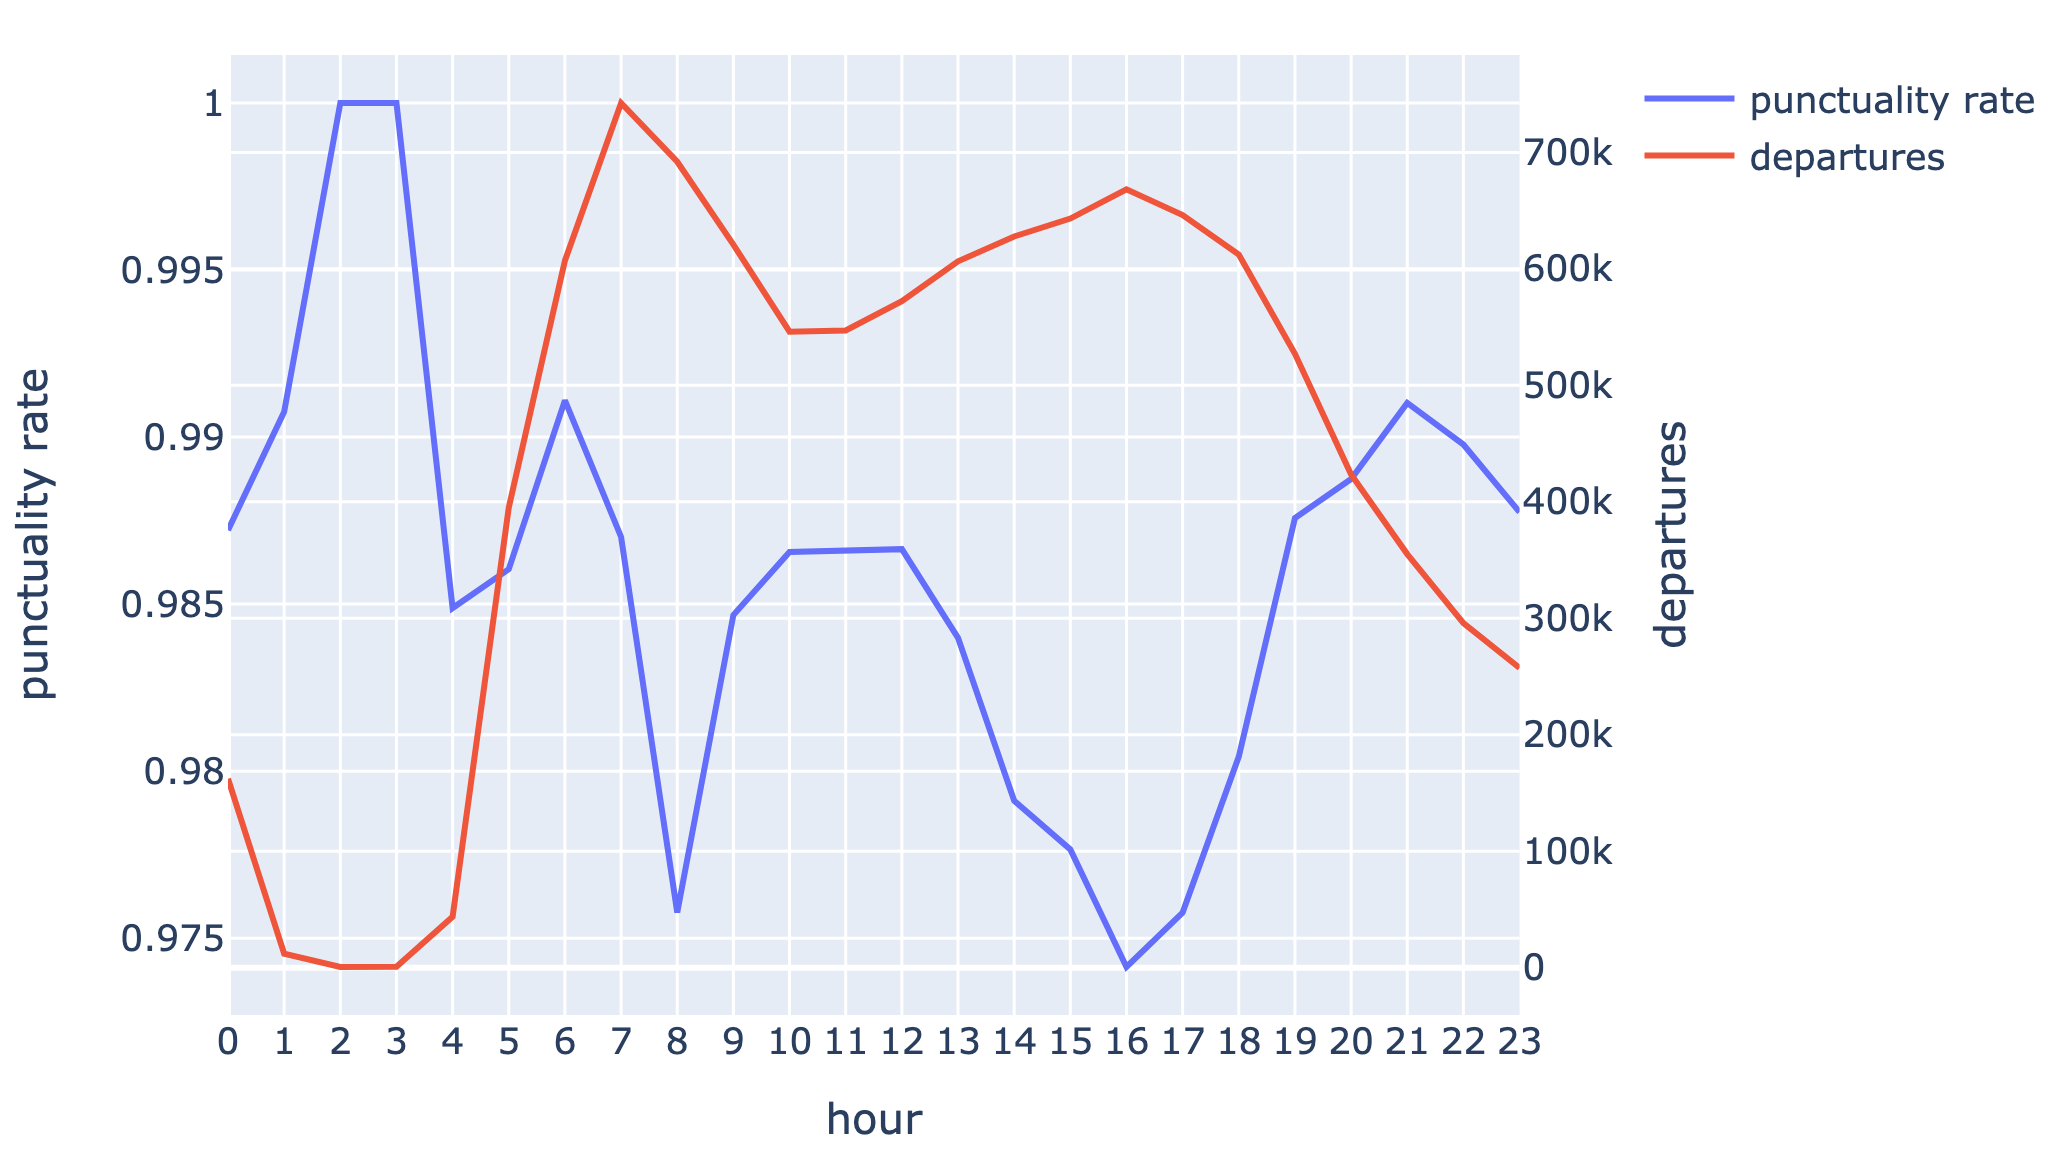
\includegraphics[width=1\textwidth]{time-of-day-weekday}
	\caption{Punctuality rate and number of departures by time of day on weekdays}
	\label{fig:time-of-day-weekday}
\end{figure}

\begin{figure}[h]
	\centering
	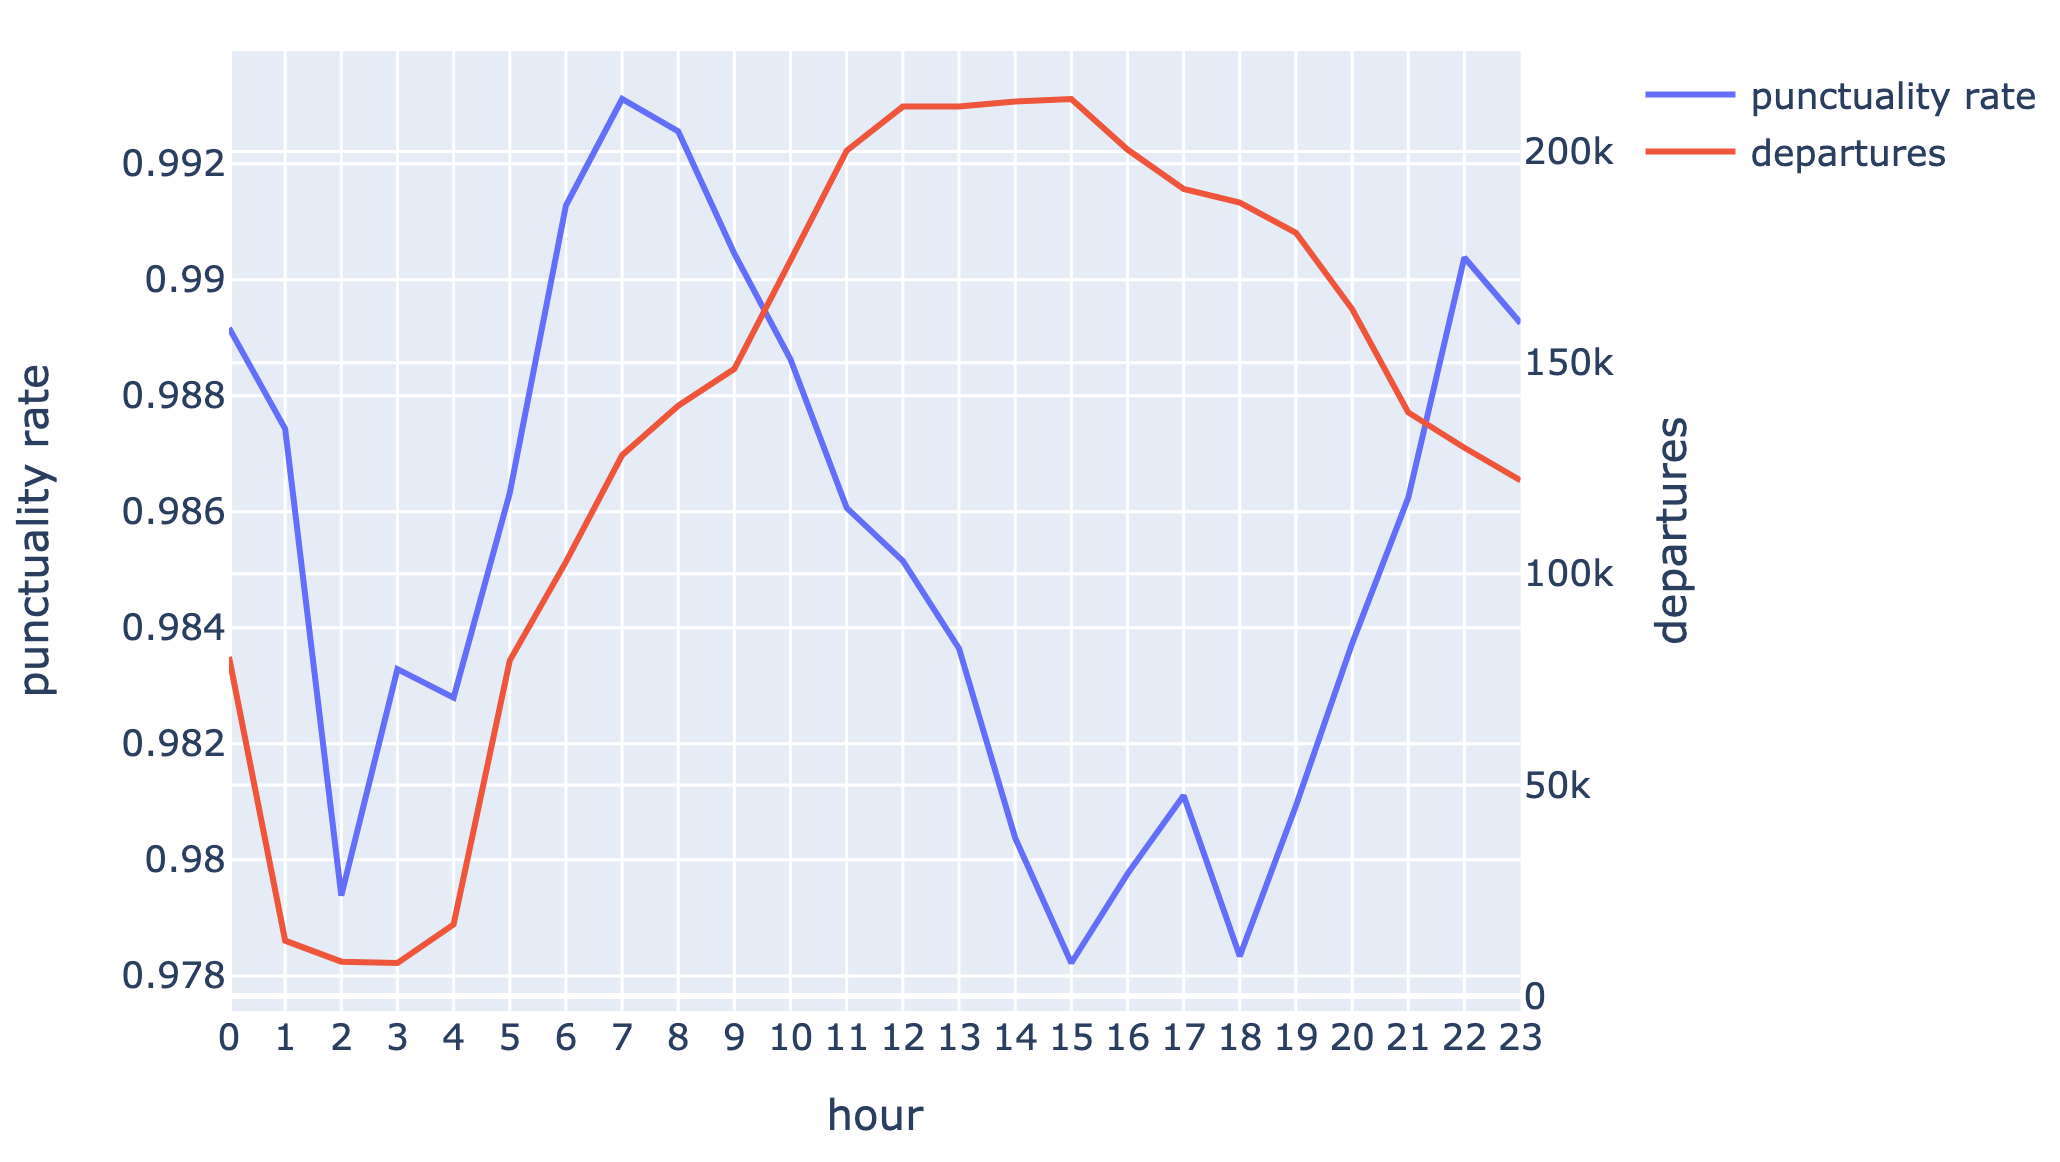
\includegraphics[width=1\textwidth]{time-of-day-weekend}
	\caption{Punctuality rate and number of departures by time of day on weekends}
	\label{fig:time-of-day-weekend}
\end{figure}

For weekdays, the punctuality rate drops significantly at \DTMtime{08:00:00} and \DTMtime{16:00:00}. During this timeframe, the number of departures also rises to the highest points, peaking at \DTMtime{07:00:00} and \DTMtime{16:00:00} with around 750,000 and 670,000 departures per hour respectively. While the amount of departures stays relatively high during midday, the punctuality rate recovers significantly. From \DTMtime{02:00:00} to \DTMtime{03:00:00} in the night, punctuality even reaches 100\%. However, on weekdays there are only limited services with only a few bus lines running, shown by the number of departures which drop to around 8000 per hour. On weekends, the image differs a lot and shows that the number of departures rises during the morning and reaches its highest point at noon, going back down at \DTMtime{15:00:00}. Further, those peaks are notably lower than on weekdays, reaching less than a third of departures with around 220,000. The punctuality rate behaves very differently too, with its lowest values being at \DTMtime{02:00:00} and \DTMtime{15:00:00}, this time reaching its maximum at \DTMtime{07:00:00}.
\section{Discussion}
\label{sec:discussion}

In this section, we will explore and discuss possible reasons for the results found in \cref{sec:analysis} and \cref{sec:visualization}.

\subsection{Line and station overview}

In \cref{sec:analysis}, we at first showed the most and least delayed lines in the network. While many lines had a perfect punctuality rate of 100\%, most of those lines are either really short or have special routes where they face very little traffic. Line 2A for example is a line that has 10 stops within the city center where traffic is rather low due to the higher number of pedestrian areas. Line ZF is a special line that travels around the Central Cemetery and thus is not affected by any traffic at all. Lines in \cref{table:overall-top10-most} that start with the letter \enquote{N} are night lines, which again face very little traffic during the night. Because of those reasons, it is not surprising that these lines have punctuality rates of 100\%. Lines 34A and 73A are also comparatively short lines, having 19 and 16 stations respectively. Additionally, many trips on those routes do not run all the way to the last station but rather end at an earlier one, resulting in trips with 10--15 stations, significantly less than the average bus route. The lines with the lowest punctuality rates all have relatively similar mean delays, ranging from 24.87 to 51.89 seconds. The least punctual line 42A, however, has a significantly higher mean delay of 149.01 seconds. Since this observation is also visible in one of the visualizations, it will be further discussed in \cref{discussion:vis}.

When looking only at metro lines, it became visible that all five lines have very high punctuality rates with the lowest value at 98.65\%. Since metro lines are entirely separated from both external traffic and each other (i.e. the individual lines do not share any tracks), those high percentages are within expectations. Excluding U6E, which is a special replacement line during construction work, all metro lines showed similar mean delays of around 10 seconds, which indicates that there are no outliers, at least when looking at the lines as a whole.

Tram lines on the other hand showed more spread-out results, which seems obvious when considering that traffic can have great effects on how smoothly a tram can operate through narrow city streets. Interestingly, the data shows that the most punctual lines are lines with fewer stops than the least punctual lines which are all relatively long lines. The five most punctual tram lines have an average of 15.8 stops, while on the other hand, the five least punctual lines have an average of 31.8 stops, offering twice as many opportunities for delayed departures and therefore being a plausible cause for those higher delay rates. An interesting observation is that three out of the five most punctual tram lines have negative mean delays. This effect is likely caused by the terminal stations, where trams have scheduled dwell times of 5--10 minutes so that the next trip can start punctually and drivers have the opportunity for a small break. Even though the negative values only occur at the terminal stations, the mean delay of the entire line is also negative. This again is a consequence of the short length of those lines. Since this especially becomes visible when looking at each stop of one line, it will be further discussed in the next section.

Next, all departures were grouped by stations and their punctuality rates were aggregated. The results showed that there is one station with significantly more delays than others. While the station in question, \textit{Blaasstraße}, is part of the second most delayed line 10A, at first sight, it is not affected by any special circumstances which could explain the drastically lower punctuality rate. This single outlier is also visible when looking at the box plots in \cref{fig:boxplot-stations}. Even when comparing the station to its direct neighbors on the line, namely \textit{Dänenstraße} and \textit{Hardtgasse}, the anomaly cannot be explained since those two stations show delay distributions in line with the overall trend. \textit{Blaasstraße} however even has a median delay of 60 seconds, whereas one would expect the median as well as the \nth{75} percentile to be 0, based on the rest of the data. To further confirm that there is no external reason for these high numbers, a local inspection and test rides on line 10A were carried out. Since this did not result in any new findings, a scheduling error or another non-obvious reason seems likely.

Looking only at stations that serve metro lines, one interesting observation is that out of the five stations with the most delays, shown in \cref{table:metro-stations-top5-least}, three have metro, tram and bus services and thus lots of transfers occurring. The five most punctual stations on the other hand, shown in \cref{table:metro-stations-top5-most}, all only serve exactly one metro line and buses, but no trams, which makes them less susceptible to delays happening due to large crowds interchanging between lines.
Overall though, all of those stations have high punctuality rates, with the difference between the most and least delayed stations only being 2.8 percentage points, which the box plot in \cref{fig:boxplot-stations} clearly demonstrates as well.

\subsection{Tram line 71 and station \textit{Karlsplatz}}

After analyzing the collected data on a more general level by looking at all lines or stations at once, \cref{sec:line-71-analysis} focused on one particular line, namely tram line 71. When looking at both punctuality rates and mean delays, one can observe that for lower punctuality rates, mean delay increases. However, for some stations such as \textit{Ring/Volkstheater U} or \textit{Oper/Karlsplatz U} this pattern does not hold, meaning that these stations have a higher mean delay than the respective next ones in the ordered list. A plausible explanation for this is that both these stations are important interchange stations for metro lines (indicated by the letter \enquote{U} in the name). At such interchanges, it is more likely that delays occur due to big crowds entering and exiting the vehicles and thus increasing dwell time. The fact that these inflated numbers do not necessarily carry on to the next stations indicates that the network operator Wiener Linien has included this fact in their schedule planning. Regarding punctuality rates, it becomes obvious that delays gathered in the city center do accumulate to the end of the line. The most punctual stations at the top of \cref{table:tram-71-stations} are all within the first few stops in the center while stations with low punctuality rates are at the end of line 71. One eye-catching exception is the last station but very first entry, \textit{Kaiserebersdorf, Zinnergasse}. While all other stations have relatively normal mean delays of 18 to 30 seconds, this station has a mean delay of -25.15 seconds. Trams in Vienna usually have a 5--10-minute stay at the terminal stations, enabling a short break for the driver and, as importantly, making up for accumulated delays and ensuring a punctual departure on the trip back. This explains the excellent punctuality rate for this particular station and likely other terminal stops as well. Since early departures are generally not desired though, there have to be more causes for this effect of negative departure delays. One of those possible causes could be that consistent intervals are preferred to perfectly following the schedule, resulting in drivers departing early for their next trip instead of waiting, which itself could cause an accumulation of waiting vehicles at the terminal station.

In addition to one single line, one station was analyzed in a similar manner, shown in \cref{table:karlsplatz-lines}. The station of choice was \textit{Karlsplatz}, as it is one of the busiest stations with metro, trams and bus lines stopping there. Metro lines again showed the highest punctuality rates and lowest mean delays. This again is most likely an effect of metros being entirely separated from other traffic, unlike trams and buses. The negative mean delay of -16.2 seconds for U2Z shows the same effect as the terminal stop of line 71 mentioned above. U2Z terminates at \textit{Karlsplatz}, meaning that it has enough leeway scheduled to make up for possible delays. In general, though, trams show worse punctuality rates and mean delays than buses at \textit{Karlsplatz}. While tram lines 71, D, 62 and 2 show consistent mean delays of around 30 seconds, line 1 has a significantly lower value with just 0.76 seconds. One possible explanation for this is that schedule planning is slightly more accurate for this line compared to the others mentioned.


\subsection{Visualizations}
\label{discussion:vis}

In \cref{sec:visualization}, two types of visualizations were presented which allow for an intuitive understanding of the large amounts of data at hand. The first one showed a map of Vienna with all stations colored on a gradient from red to green, respective to their punctuality rate. A sequence of bus stops on line 42A was visibly more yellow than the rest of the network. Line 42A is a rather short line with twelve stops, none of which are located within the inner districts, where more traffic and passenger volume would be expected. While previous delays do accumulate towards the end of a line as seen in previous sections, it is interesting to see the effect this strongly at this line and leaves the question if there exist other reasons for this behavior.

The same visualization but with only metro and tram stations shown discovered that the stations \textit{Gredlerstraße} and \textit{Marsonogasse} were the two most delayed tram stations in the network. While the former is a regular station part of line 2 (one of the most delayed trams), the latter is a special station located at one of the tram depots, where vehicles only stop at the very beginning and end of service. In \cref{fig:metro-only-stations}, where only metro stations are shown, it became again apparent that delays that accumulate through the trip of a metro line are accounted for at the terminal stop by calculating time reserves accordingly. This pattern is visible at most terminal stops, where their immediate neighbors show a considerably lighter shade of green or even reaching to the end of the color scale like for the U2 station \textit{Aspern Nord}, located in the far east of Vienna.

For the next visualization, all departures were grouped by the hour of the day and then plotted onto a line graph with both the mean delay and the number of departures visible. In order to see the potential effect of rush hour traffic more clearly, the departures were split into weekdays and weekends and visualized separately. This effect was indeed clearly visible, especially on weekdays when the punctuality rate was significantly lower at \DTMtime{08:00:00} and \DTMtime{16:00:00}. On Saturdays and Sundays however, the image was very different, not showing any rush hours but with minimums at \DTMtime{02:00:00} and \DTMtime{15:00:00}.
\section{Conclusion}
\label{sec:conclusion}

This section will conclude and summarize the results by highlighting key takeaways and putting them into the context of the scope and goals of this thesis. Finally, aspects that were not in the scope of this thesis and are subject to further research will be mentioned.

The aim of this thesis was to analyze the public transport network of Vienna for on-time performance and detect potential delay hotspots where punctuality rates are particularly low. Public transport is one of the key factors of a functioning livable city and good on-time performance is of high importance in order to ensure high usage and passenger satisfaction. In order to conduct this analysis, a custom data collection script was written which persisted 13.7 million departure records over a period of 30 days. Next, the collected data was cleaned up and filtered for incomplete or irrelevant results. For the following analysis, the data was either further filtered in order to highlight certain aspects, or it was aggregated and summarized as a whole.

Evaluating the data showed that the network offers a very good general on-time performance. While metro lines usually had very few delays due to their separation from other traffic, bus lines had both the highest and lowest punctuality rates, depending on their specific route. The initial assumption was that delays occur more often at busy interchange stations due to lots of passengers getting on and off the vehicles. This assumption did not hold in the general case, as the lowest punctuality rates were found at regular bus stations. On certain lines, however, this effect did become visible, like on tram line 71, which was analyzed in more detail in \cref{sec:line-71-analysis}. Other expected delay hotspots were terminal stations since those provide the opportunity for previously collected delays to accumulate. An interesting observation regarding this was that the terminal stops themselves surprisingly showed the best punctuality rates and even negative mean delays. However, the last 3--5 stops before them had in fact relatively low punctuality rates, suggesting that previous delays do accumulate but are however accounted for by including a leeway in the schedule. Lastly, there were some stations and even parts of whole lines that showed substantially lower punctuality rates than others. In contrast to the aforementioned cases, these however did not show any apparent systemic reason for the bad on-time performances.

In addition to the analysis done in \cref{sec:analysis}, visualizations of the delay data were presented in \cref{sec:visualization}. The aim of those visualizations was to provide an intuitive understanding of the data. The first visualization was a city map with stations plotted at their locations. Each station was colored on a gradient ranging from green to red which represents its punctuality rate. With this, the already known results from \cref{sec:analysis} were visualized as well as new delay hotspots discovered. Next, a line graph was presented which showed the number of departures and the punctuality rate per hour of the day, separated for weekdays and weekends. This showed the expected result that on-time performance drops significantly for morning and afternoon rush hour traffic during weekdays.

The presented statistics and graphics showed that there is definitely room for improvement in Vienna's public transport network, albeit the overall results suggest that there are already various measures put into practice to avoid long delays and with that unsatisfied passengers.

\subsection{Future Work}
\label{sec:future}

There are many opportunities for further analysis of departure and in particular delay data, both in other cities and in Vienna. While the scope of this thesis was limited to departure delays, arrival delays could be analyzed and used in calculations combining arrival and departure times. For example, dwell times---another important measure in public transport analysis---could be calculated and analyzed. With dwell times, stations that actually cause delays could be detected better than when using only departure delays since one can see whether a delay was just carried on from the previous station (indicated by a normal, short dwell time) or a delay emerged at the station in question (indicated by a higher than expected dwell time). Of course, delays can also occur between stations, where this method would not be viable.

As mentioned in previous sections, another important indicator of on-time performance is the intervals between departures. When there are a lot of delays but consistent intervals, passengers are still satisfied if intervals are sufficiently short \autocite[378]{van-oort-2015}. It could be studied how intervals differ from their schedule in order to detect possible delay hotspots. In combination with passenger surveys which could determine acceptable interval deviations, identified hotspots can be narrowed down to a few high-priority locations, where shorter intervals would result in the highest increase in customer satisfaction. Additionally, passenger volume should be taken into consideration. After all, very short intervals are only economically viable if they meet passenger demand.

In addition to the visualizations presented in this thesis, interactive visualizations could be explored in order to provide the reader with even more relevant data and a more engaging experience than a static graph or image. With location data, a live map showing the position of vehicles in real-time would be an interesting interactive application. Even without location data, one could in theory calculate vehicle locations by multiplying the expected minutes or seconds until arrival by the average speed of the vehicle. Naturally, this method can only provide estimations, combined with smooth interpolation and animations this could however result in a useful, visually appealing visualization.

In order to improve the network and the situation for passengers, it is important that after the on-time performance has been studied, concrete measures are implemented that try to resolve identified problems. This can be done by both the transit company which can for example improve vehicles, driver behavior or station infrastructure and also by the city itself and its traffic planning, for example by reducing car lanes in order to avoid delays caused by traffic blocking buses or trams. 

 % the main text

%\input{acknowledgements}

\ifmmtpaper

\printbibliography

\else % only use the following for thesis format

\newpage

\printbibliography

\fi


 % group open
\ifmmtpaper 
\begingroup 
    % is required because paper template messes with sizes
    \fontsize{12}{18}\selectfont        
    \setlength{\parindent}{0pt}
    \setlength{\parskip}{5pt plus 2pt minus 1pt}
    \sectionfont{\fontsize{14}{15}\selectfont}
\fi

\ifmmtpaper\else % nicht im paper

\newpage
\onecolumn
\begin{appendices}

%\renewcommand{\thesubsection}{\Alph{subsection}}
\section{git-Repository}

According to the respective guidelines.

The repository must be uploaded to the MMT/HCI git server {\url{gitlab.mediacube.at}}

{\color{red}\url{https://gitlab.mediacube.at/fhs45907/bachelor-thesis}}
	

% DIESEN TEIL NICHT LÖSCHEN ODER ÄNDERN == BEGINN
%\fi % end if for the if \ifmmtreviewversion 
\end{appendices}
% DIESEN TEIL NICHT LÖSCHEN ODER ÄNDERN == ENDE


\fi

% group closing
\newpage

This work has the following word count (counted by texcount): 
%TC:ignore
\detailtexcount{body}
%TC:endignore

\end{document}
